% Session 3: Optimal Carbon Taxes with Deep Surrogates
% Main part: the design operator (constrained optimal taxes and transfers,
% Kubler/Scheidegger/Surbek); appendix: the quantify operator (UQ of the SCC,
% Friedl/Kubler/Scheidegger/Usui) plus model, calibration, and DEQN/GP details.
\documentclass[10pt,aspectratio=169]{beamer}

\usepackage[utf8]{inputenc}
\usepackage[T1]{fontenc}
\usepackage{lmodern}
\usepackage{amsmath, amssymb, amsthm}
\usepackage{booktabs}
\usepackage{graphicx}
\usepackage{hyperref}
\usepackage{tikz}
\usepackage{xcolor}

% == Lazy extensions required by ported frames (definitions from deck_tax.tex) ==
\usepackage{natbib}
\usepackage{bm}
\usepackage{makecell}
\usepackage{tabularx}
\usepackage[font=footnotesize,labelfont=bf]{caption}
\usepackage[font=footnotesize,labelfont=bf]{subcaption}
\usepackage{pgfplots}
\usepgfplotslibrary{fillbetween}
\pgfplotsset{compat=1.18}
\usetikzlibrary{positioning,calc,arrows}

\graphicspath{{assets/}}

\setbeamertemplate{footline}{
  \hfill
  \insertframenumber\,/\,\inserttotalframenumber\kern1em\vskip4pt}
\setbeamerfont{frametitle}{size=\huge}

% Color setup mirrored from Session 2 (course master).
% NOTE: deck_tax.tex defines uzhblue twice (RGB 0,40,165 and rgb 0,0,0.5);
% defined exactly once here, with the course value (see open_questions.md).
\definecolor{uzhblue}{RGB}{0, 40, 165}
\definecolor{uzhgreylight}{RGB}{235, 235, 235}
\definecolor{darkred}{RGB}{170, 0, 0}
\definecolor{softblue}{RGB}{60, 100, 200}
% Additional colors required by ported tax-deck frames
\definecolor{uzhorange}{RGB}{220,96,39}
\definecolor{uzhgrey}{RGB}{163,173,186}
\definecolor{uzhgreydark}{RGB}{81.5,86.5,94}

\newcommand{\E}[1]{\mathbb{E}\!\left[#1\right]}
\newcommand{\emphc}[1]{\textbf{\textcolor{darkred}{#1}}}
% UQ-deck emphasis macros, remapped onto the course palette (see CHANGELOG.md)
\newcommand{\key}[1]{\textbf{\textcolor{uzhblue}{#1}}}
\newcommand{\keyc}[1]{\textcolor{uzhblue}{#1}}
\newcommand{\stoch}[1]{\textcolor{darkred}{#1}}

\setbeamercolor{title}{fg=uzhblue}
\setbeamercolor{frametitle}{bg=uzhgreylight, fg=uzhblue}
\setbeamercolor{block title}{bg=uzhblue, fg=white}
\setbeamercolor{block body}{bg=uzhgreylight, fg=black}
\setbeamercolor{block title alerted}{bg=darkred, fg=white}
\setbeamercolor{block body alerted}{bg=uzhgreylight, fg=darkred}

\DeclareMathOperator*{\argmin}{arg\,min}
\DeclareMathOperator*{\argmax}{arg\,max}

% Appendix frame-number bookkeeping (from deck_tax.tex)
\newcommand{\backupbegin}{
   \newcounter{framenumberappendix}
   \setcounter{framenumberappendix}{\value{framenumber}}
}
\newcommand{\backupend}{
   \addtocounter{framenumberappendix}{-\value{framenumber}}
   \addtocounter{framenumber}{\value{framenumberappendix}}
}

\title[PKU--Zurich Summer School 2026]
{PKU--Zurich PhD Summer School on Machine Learning for Macroeconomics and Finance}
\subtitle{Optimal carbon taxes with deep surrogates --- solve once, ask many questions}
% Alternative subtitles:
% "From estimation to decisions: uncertainty quantification and optimal carbon taxes on one deep surrogate"
% "Three questions, one surrogate: estimating, quantifying, and designing with deep equilibrium nets"
\author{Simon Scheidegger \and Felix K\"ubler}
\institute{HEC Lausanne $\cdot$ University of Zurich}
\date{July 6--10, 2026 \,$\cdot$\, Beijing, China}

\begin{document}

% =====================================================================
% Section 0: Title, roadmap, learning objectives
% =====================================================================
% TIMING: cumulative 0 min when this section starts

% == F1: Title slide ==
{\setbeamercolor{background canvas}{bg=uzhgreylight}
\begin{frame}
\titlepage
\vspace{-0.3cm}
\begin{center}
{\footnotesize \url{https://liboecon.com/2026_summer_school.html}}
\end{center}
\end{frame}
}

% == F2: Roadmap ==
\begin{frame}{Roadmap of This Lecture}
\small
\begin{enumerate}
    \item \textbf{Where Session 2 left us.} One trained surrogate, one question answered (estimation); two questions still open.
    \vspace{0.2em}
    \item \textbf{The two-surrogate pipeline, generalized.} Pseudo-states $(\bm{\theta}, \vartheta)$, quantities of interest that generalize $m(\theta)$, and three post-processing operators.
    \vspace{0.2em}
    \item \textbf{Design: constrained optimal carbon taxes.} Taxes and transfers in a stochastic OLG IAM: three policy scenarios, from unconstrained to Pareto-improving.
    \vspace{0.2em}
    \item \textbf{Synthesis.} One surrogate, three questions; practical guidance; extensions and open questions.
    \vspace{0.2em}
    \item \textbf{Appendix: Quantify.} Uncertainty quantification of the social cost of carbon (univariate effects, Sobol' indices, Shapley values), plus model and calibration details.
\end{enumerate}
\end{frame}

% == F3: Learning objectives ==
\begin{frame}{Learning objectives}
\textbf{By the end of this lecture you should be able to:}
\begin{itemize}
  \item Extend pseudo-state surrogates from estimation to uncertainty quantification and policy design
  \item Compute the social cost of carbon and welfare quantities of interest from surrogate simulations
  \item Rank parameter uncertainties via univariate effects, Sobol' indices, and Shapley values
  \item Add a Gaussian process and Bayesian-active-learning layer when each QoI evaluation needs heavy Monte Carlo
  \item Solve constrained policy problems, including Pareto constraints, directly on the surrogate
\end{itemize}
\end{frame}

% =====================================================================
% Section 1: Motivation: from estimation to two new questions
% =====================================================================
% TIMING: cumulative 4 min when this section starts
\section{Motivation}

% == F4 [NEW, L15: Wrap-Up + Bridge] ==
\begin{frame}{Where Session 2 Left Us}
\small
\begin{columns}[c]
\begin{column}{0.62\textwidth}
\textbf{This morning's takeaways:}
\begin{itemize}\itemsep2pt
  \item A neural surrogate with parameters as \emph{pseudo-states} decouples the cost of solving the structural model from the cost of moment-matching.
  \item Train once, use it inside any optimizer: millions of cheap moment evaluations under common random numbers.
  \item Joint estimation made the \emph{identification ridge} visible; the interior-solution check closed the loop.
\end{itemize}
\vspace{0.3em}
\textbf{The pivot:} estimation treats $\bm{\theta}$ as unknown but \emphc{fixed}. Two questions remain:
\begin{itemize}\itemsep2pt
  \item What if $\bm{\theta}$ \emphc{stays uncertain} after all we know?
  \item What if some inputs are not parameters at all, but \emphc{choices}?
\end{itemize}
\vspace{0.3em}
Today's mantra: \emphc{solve once, ask many questions.}
\end{column}
\begin{column}{0.36\textwidth}
\centering
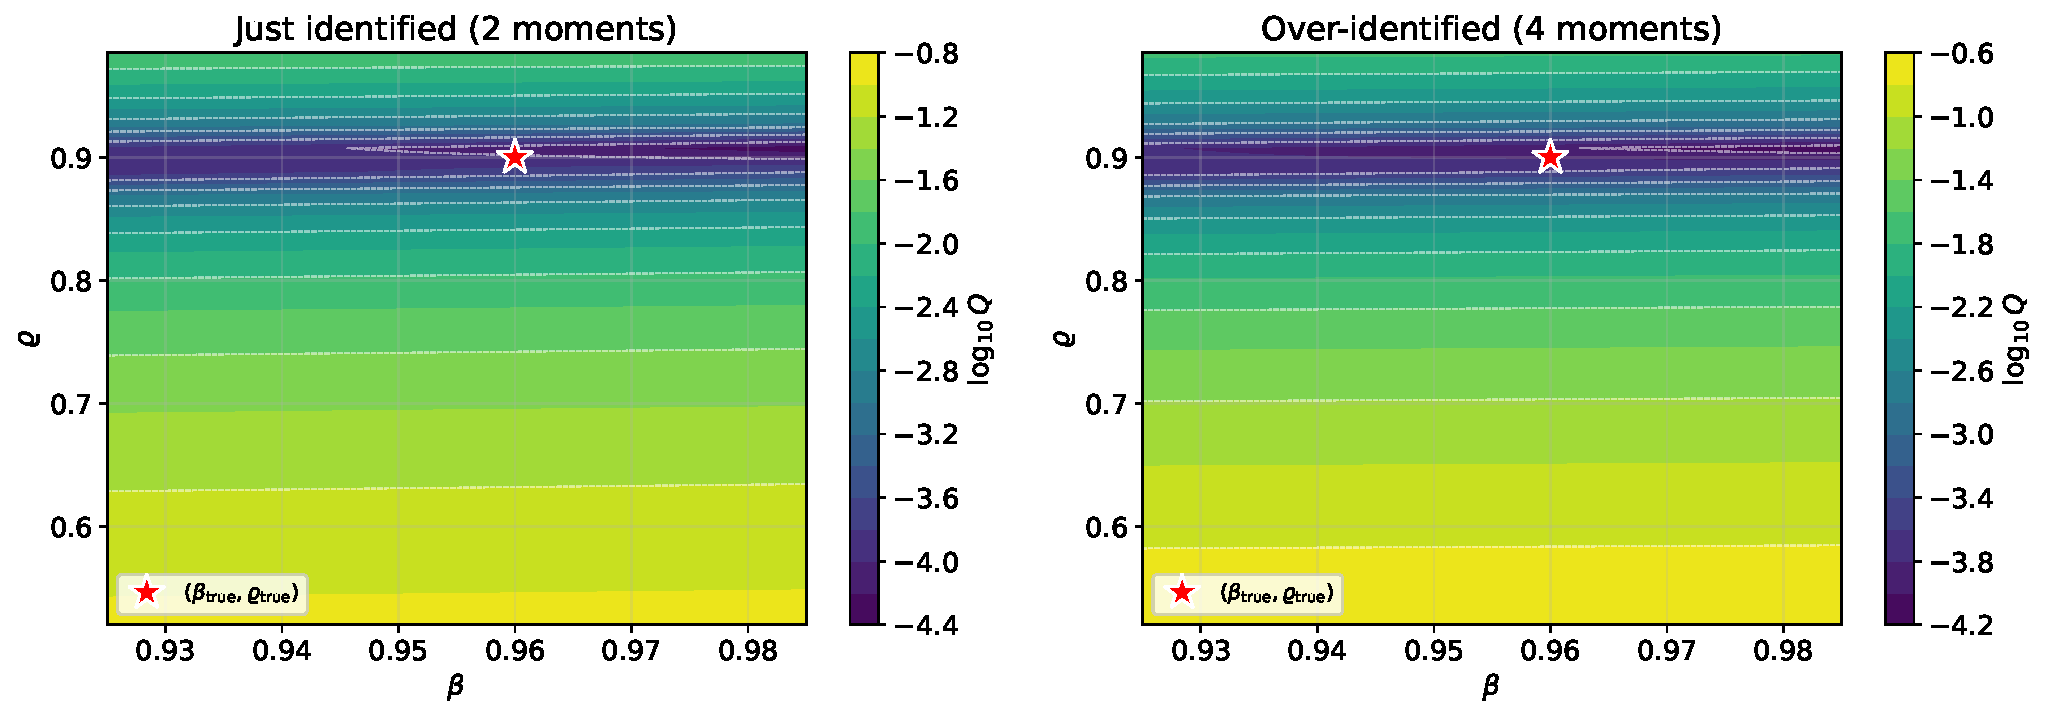
\includegraphics[width=\linewidth]{l15/joint_criterion_contour.pdf}
{\scriptsize Session 2's identification ridge: the criterion's shape, not its argmin, carried the lesson.}
\end{column}
\end{columns}
\end{frame}

% == F5 [NEW]: thesis frame ==
\begin{frame}{Three Operators, One Surrogate}
\small
Three questions ride on one parametric surrogate. Session 2 asked the first; today we work out \emphc{design} in full --- the appendix works out \emphc{quantify}.
\vspace{0.5em}
\begin{center}
\footnotesize
\begin{tabular}{p{0.09\textwidth}p{0.23\textwidth}p{0.36\textwidth}p{0.17\textwidth}}
\toprule
\textbf{Operator} & \textbf{Question} & \textbf{Post-processing} & \textbf{Where} \\
\midrule
\emphc{Estimate} & Which parameters fit the data? & $\argmin$ of an SMM criterion over $\bm{\theta}$ & Session 2 \\[3pt]
\emphc{Quantify} & Which parameter uncertainties matter? & propagate $p(\bm{\theta})$ through a QoI: univariate effects, Sobol' indices, Shapley values & Appendix (SCC) \\[3pt]
\emphc{Design} & Which policy is best? & constrained $\argmax$ of a welfare QoI over $\vartheta$ & Today (carbon taxes) \\
\bottomrule
\end{tabular}
\end{center}
\vspace{0.5em}
Identical machinery throughout: the \emphc{two-surrogate pipeline}. Surrogate 1 solves the equilibrium over states and pseudo-states; Surrogate 2 maps parameters to quantities of interest. Only the post-processing operator changes.
\end{frame}

% == F6 [TAX: The Challenge: Climate Risk & Heterogeneity] ==
\begin{frame}{The Challenge: Climate Risk \& Heterogeneity}
    \begin{columns}[c]
        \begin{column}{0.45\textwidth}
            \centering
            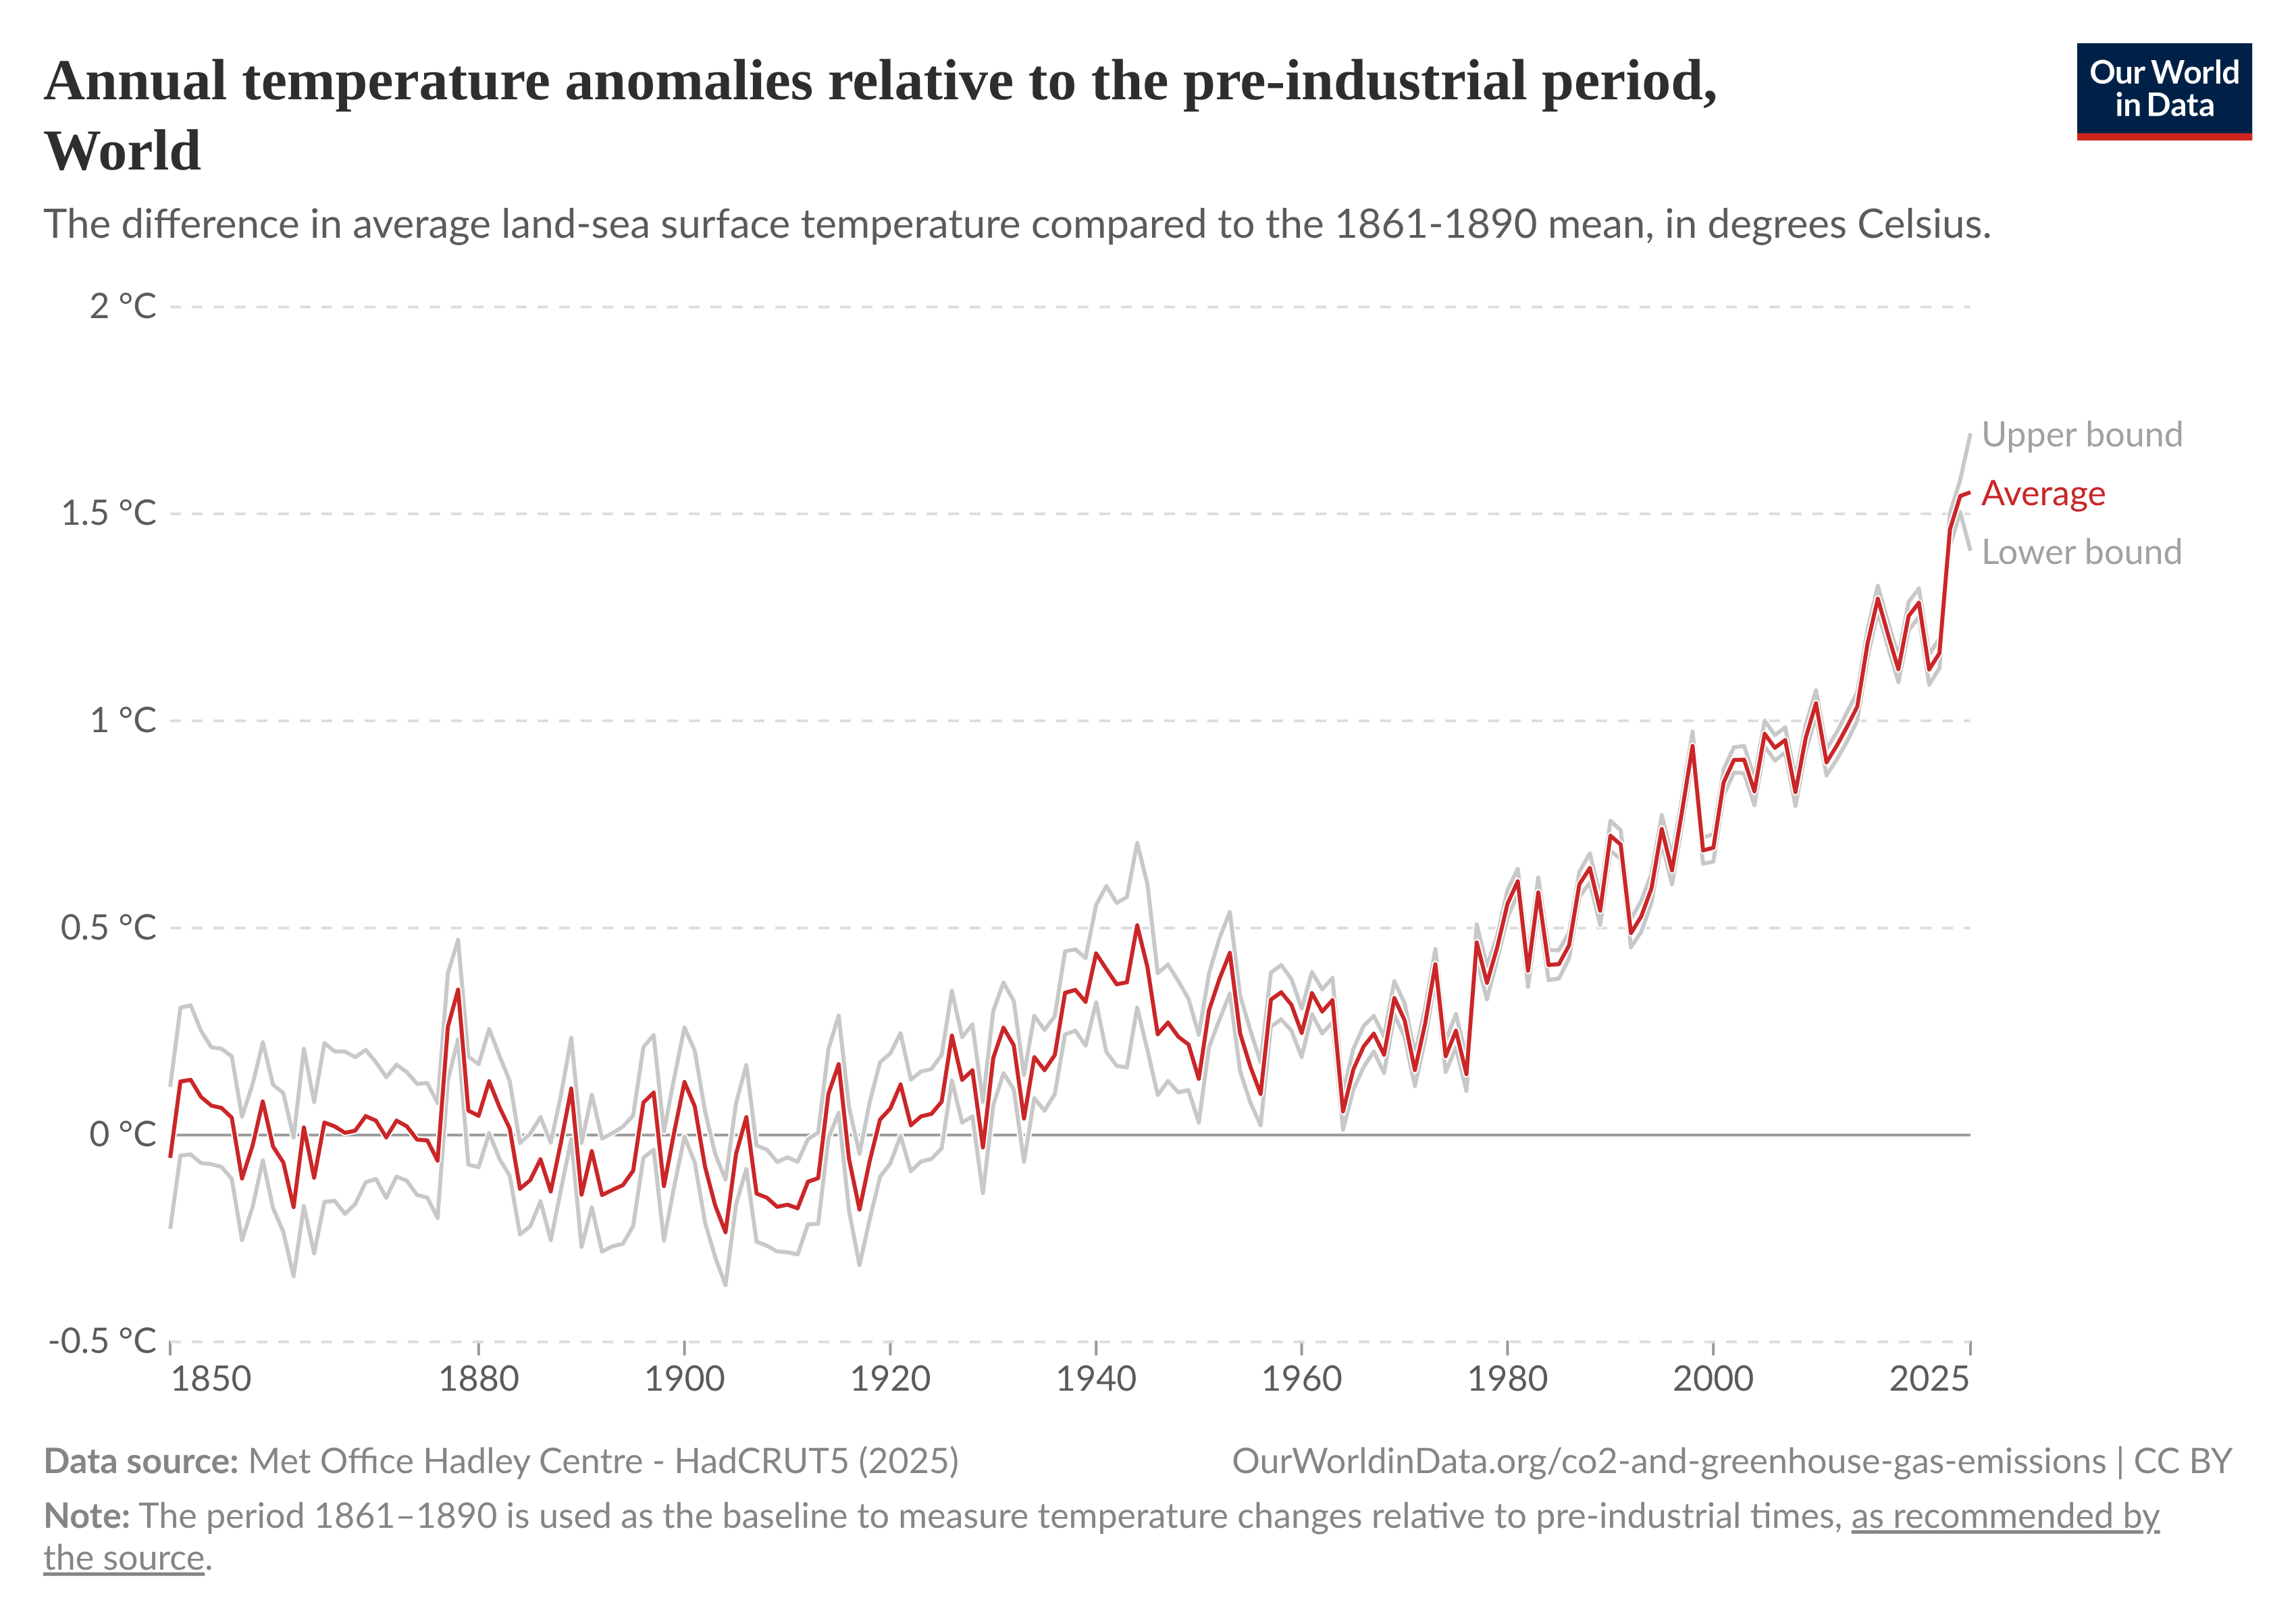
\includegraphics[width=0.85\linewidth]{tax/temperature-anomaly.png}

            \vspace{0.4em}

            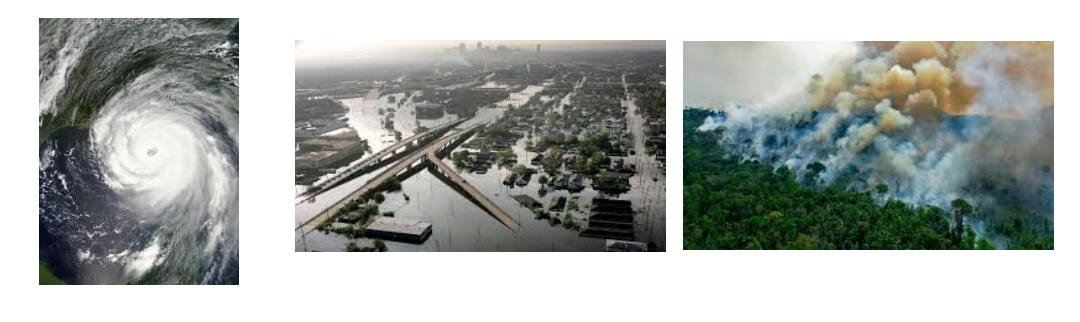
\includegraphics[width=0.85\linewidth]{tax/global-warming.png}
        \end{column}
        \begin{column}{0.55\textwidth}
            \small
            \begin{itemize}
                \setlength\itemsep{0.8em}
                \item \textbf{Systemic Risk:} Climate change poses a fundamental threat to global economic stability and human welfare.
                \item \textbf{Non-Linear Dynamics:} Tipping points introduce the risk of irreversible, catastrophic environmental shifts.
                \item \textbf{Distributional Impact:} Effects will be highly heterogeneous, creating profound equity challenges across regions and generations.
                \item \textbf{Literature Context:} These macro-financial linkages are detailed in the recent review Fernandez-Villaverde, Gillingham, and Scheidegger (2025).
            \end{itemize}
        \end{column}
    \end{columns}
\end{frame}

% == F7 [NEW, merge: UQ motivation + TAX motivation] ==
\begin{frame}{Two Policy Questions, One Computational Wall}
\footnotesize
\begin{columns}[t]
\begin{column}{0.48\textwidth}
\textbf{Quantify: how uncertain is the SCC?} {\tiny (worked out in the appendix)}
\begin{itemize}\itemsep3pt
  \item \key{Carbon taxation}: widely supported policy response to the climate change problem.
  \item The level of the carbon tax is based on the social cost of carbon (SCC): the marginal loss caused by an extra ton of CO$_2$ emissions.
  \item SCC values are computed with \key{integrated assessment models} (IAMs) that link economy and climate.
  \item IAMs are subject to \key{significant parametric uncertainty, model uncertainty, and climate risks of tipping points}.
\end{itemize}
\end{column}
\begin{column}{0.48\textwidth}
\textbf{Design: which carbon tax is best?}
\begin{itemize}\itemsep3pt
  \item \textbf{The Consensus:} Carbon pricing is widely regarded as the most efficient tool to mitigate emissions.
  \item \textbf{The Difficulty:} In a world with heterogeneous agents (e.g., OLG), simple taxes create winners and losers, threatening political feasibility.
  \item \textbf{The Objective:} A systematic way to compute \textcolor{blue}{constrained optimal taxes} that account for stochastic risks (tipping points) and respect political constraints (Pareto improvements): most work relies on \textcolor{blue}{simplifying assumptions} or heuristic ``guessing''.
\end{itemize}
\end{column}
\end{columns}
\vspace{0.6em}
\emphc{The wall:} both questions need thousands of model evaluations. IAMs are complex non-linear models highly susceptible to the curse of dimensionality; evaluating expected welfare requires 10{,}000 Monte Carlo paths per policy $\vartheta$. Session 2's answer carries over: with a deep surrogate, the inner loop is three orders of magnitude cheaper.
\end{frame}

% =====================================================================
% Section 2: The two-surrogate pipeline, generalized
% =====================================================================
% TIMING: cumulative 12 min when this section starts
\section{The pipeline, generalized}

% == F8 [TAX: Our Novel Approach in a Nutshell, rebuilt in Session 2 language] ==
\begin{frame}{The Two-Surrogate Pipeline in a Nutshell}
\small
  \begin{itemize}
    \item \textbf{Step 1: Global solution with DEQN (Surrogate 1)}
      \begin{itemize}
        \item \textcolor{blue}{Solve the model as a function of states and pseudo-states in one go}: train on $\tilde{x} = (x, \bm{\theta}, \vartheta)$, exactly the pseudo-state trick of Session 2.
        \item \textcolor{blue}{For linear tax rules in cumulative emissions, $\kappa$, $TP$}: 4 tax pseudo-states $\vartheta = (\vartheta_0, \vartheta_E, \vartheta_\kappa , \vartheta_{TP})$, plus \textcolor{blue}{12 from transfer shares}.
      \end{itemize}
      $\Rightarrow$ \textcolor{blue}{Once trained, the solution allows us to simulate data essentially for free}.
    \item \textbf{Step 2: Simulate quantities of interest (Surrogate 2 where needed)}
      \begin{itemize}
        \item $\widehat{\mathrm{QoI}}(\cdot)$ generalizes Session 2's moment map $m(\theta)$: in Session 2 three moments; today 40 cohort welfares, and in the appendix the SCC.
        \item Where one QoI evaluation needs heavy Monte Carlo, fit a Gaussian process with Bayesian active learning over the parameters.\footnote{A surrogate is a 21st-century lookup table: Welfare($\vartheta_1,\cdots,\vartheta_N$).}
      \end{itemize}
    \item \textbf{Step 3: Post-process}
      \begin{itemize}
        \item Estimate ($\argmin$), quantify (global sensitivity analysis), or design (constrained $\argmax$): three operators on the same object.
      \end{itemize}
  \end{itemize}
\end{frame}

% == F9 [TAX: Recall: Steps of the Method (2 Surrogates)], annotated ==
\begin{frame}{Recall: Steps of the Method (2 Surrogates)}
     \begin{figure}
 \centering
 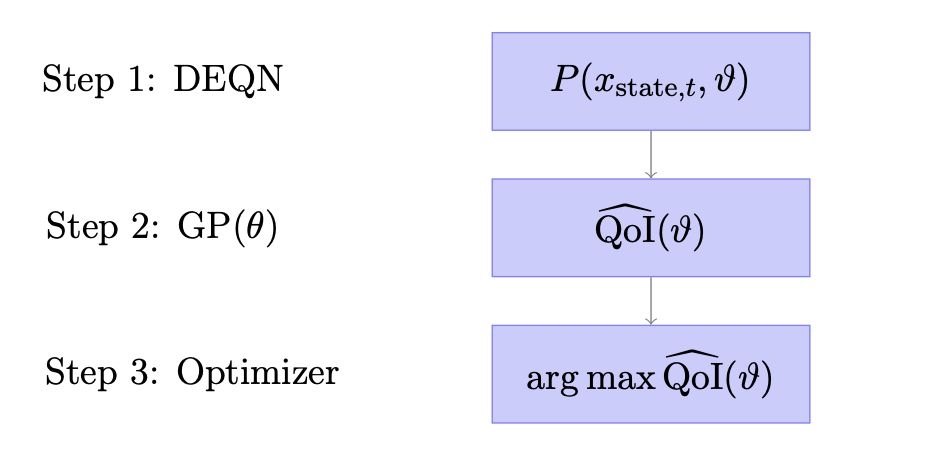
\includegraphics[width=0.72\textwidth]{tax/flow_chart_2.png}
 \end{figure}
 \vspace{-0.4em}
 \begin{center}
 \small The final box branches into the three operators: \emphc{estimate} ($\argmin$, Session 2) $\cdot$ \emphc{quantify} (global sensitivity analysis, appendix) $\cdot$ \emphc{design} (constrained $\argmax$, today).
 \end{center}
\end{frame}

% == F10 [TAX: Deep equilibrium nets], the single recap; carries callback (a) ==
\begin{frame}{Recap: Deep Equilibrium Nets (assumed known)}
\small
{A \textbf{functional rational expectations equilibrium}: $\{f_i\}_{i=1}^{N_{\mathrm{out}}}$, where
\begin{align}
f_i&: \mathcal{D} \subset \mathbb{R}^{N_{\mathrm{in}}} \rightarrow \mathbb{R}: \underbrace{x}_{\text{state}} \rightarrow \underbrace{f_i(x)}_{\text{endogenous variables}} \text{, s.t.}:  \underbrace{\textbf{G}(x, f_1, \dots, f_{N_{\mathrm{out}}})= 0}_{\text{equilibrium conditions}} \nonumber
\end{align}}
{{A \textbf{deep equilibrium net}: $\mathcal{N}_{\bm{\rho}}$, with
$\mathcal{N}_{\bm{\rho}} : \mathcal{D} \subset \mathbb{R}^{N_{\mathrm{in}}} \rightarrow \mathbb{R}^{N_{\mathrm{out}}}$, trained so that
$\mathcal{N}_{\bm{\rho}}(x) \approx (f_1(x), \dots, f_{N_{\mathrm{out}}}(x))$
by minimizing the implied error in the equilibrium conditions along simulated paths \citep{azinovic_et_al_2019}.\footnote{Sample codes: \url{https://github.com/sischei/DeepEquilibriumNets}. Loss function, training loop, and architecture details: appendix.}}}

\vspace{0.4em}
\begin{block}{Callback to Session 2}
In Session 2 the QoI was the moment vector $m(\theta)$ and the operator was $\argmin$; today the QoIs are the SCC and cohort welfares, and the operators change.
\end{block}

\vspace{0.2em}
{\footnotesize \emph{Notation.} On Day 2, $\theta$ denoted the network weights; today $\bm{\theta}$ is reserved for structural parameters, so the network weights are $\bm{\rho}$.}
\end{frame}

% == F11 [NEW]: what scales up ==
\begin{frame}{What Scales Up Relative to Session 2}
\small
\begin{center}
\begin{tabular}{p{0.21\textwidth}p{0.33\textwidth}p{0.36\textwidth}}
\toprule
 & \textbf{Session 2 (Brock--Mirman)} & \textbf{Today (climate applications)} \\
\midrule
Surrogate 1 inputs & $(z, K, \varrho)$, then $(z, K, \beta, \varrho)$ & OLG IAM state $[t, TP_t, TP_{\mathrm{reached}}, \kappa_t, a_{t,j}, E_t]$ plus 16 policy pseudo-states; IAM state plus uncertain $\bm{\theta}$ in the UQ appendix \\[3pt]
QoI shape & three scalar moments $m_1, m_2, m_3$ & an SCC surface $\mathrm{SCC}(\theta_1,\dots,\theta_N)$ and 40 cohort welfares \\[3pt]
Second surrogate & none needed: moments were cheap & GP regression + Bayesian active learning: each welfare evaluation costs 10{,}000 simulated paths \\
\bottomrule
\end{tabular}
\end{center}
\vspace{0.4em}
\textbf{Cost that does not scale up:} Surrogate 1 trains in about 4h from scratch on a laptop, minutes when warm-started; Surrogate 2 needs only 500 simulations (450 Latin hypercube + 50 actively learned).
\end{frame}

% == F12 [NEW]: operators formally (definitions only, no empirics) ==
\begin{frame}{Post-Processing: Three Operators, Formally}
\footnotesize
\textbf{Estimate (Session 2, for continuity).}
\[
    \widehat\theta_{\text{SMM}} \;=\; \argmin_{\theta} \;
        \bigl[\widehat g_T - \widehat m_S(\theta)\bigr]^{\!\top}\, W \;
        \bigl[\widehat g_T - \widehat m_S(\theta)\bigr]
\]
\textbf{Quantify (appendix).} For a QoI $Y = \mathcal{M}(\bm{\theta})$ with uncertain $\bm{\theta} \sim p(\bm{\theta})$:
\[
  \underbrace{\mathcal{M}^{1}_{i}(t) = \mathbb{E}_{\theta_{-i}}\!\left[ Y \mid \theta_{i}=t \right]}_{\text{univariate effect}}
  \qquad
  \underbrace{S_{i} = \frac{\mathrm{Var}_{\theta_{i}}\!\left[ \mathbb{E}\left[ Y \mid \theta_{i} \right] \right]}{\mathrm{Var}\left[ y \right]}, \quad
  S^{T}_{i} = \frac{\mathbb{E}_{\theta_{-i}}\!\left[\mathrm{Var}\left[ Y \mid \theta_{-i} \right]\right]}{\mathrm{Var}\left[ y \right]}}_{\text{first-order and total Sobol' indices}}
  \qquad
  \underbrace{Sh_{i}}_{\substack{\text{Shapley value: fair attribution} \\ \text{of } \mathrm{Var}(\mathrm{QoI}) \text{ across parameters}}}
\]
\textbf{Design (today).} For a welfare QoI over policy parameters $\vartheta$:
\[
   \vartheta^* = \argmax_{\vartheta} \widehat{\mathrm{QoI}}(\vartheta)
   \quad \text{s.t. feasibility and, if imposed, Pareto constraints.}
\]
\vspace{0.1em}
Same surrogate under all three operators; only the question changes.
\end{frame}

% == F13 [NEW, short]: today's two instantiations ==
\begin{frame}{Today's Instantiations}
\begin{block}{Main part: Design}
$\vartheta$ = tax and transfer parameters $\cdot$ QoI = 40 cohort welfares $\cdot$ operator = constrained $\argmax$.
\end{block}
\vspace{0.8em}
\begin{block}{Appendix: Quantify}
$\bm{\theta}$ = structural parameters (preferences, damages, climate sensitivity) $\cdot$ QoI = the social cost of carbon $\cdot$ operator = global sensitivity analysis.
\end{block}
\end{frame}

% =====================================================================
% Section 3 (main): constrained optimal carbon taxes
% =====================================================================
% TIMING: cumulative 48 min when this section starts
\section{Constrained optimal carbon taxes}

% == F26: divider ==
{\setbeamercolor{background canvas}{bg=uzhgreylight}
\begin{frame}
\Huge \textcolor{uzhblue}{Optimal Carbon Taxes and Transfers}
\end{frame}}

% == F27 [TAX: Overview of our Stochastic IAM] ==
\begin{frame}[fragile]{Overview of our Stochastic IAM}
\begin{itemize}
    \item 12 Overlapping generations of selfish agents.
            \vspace{0.4cm}
    \item 5-yearly-calibrated model: agents live from age 20 to age 80.
            \vspace{0.4cm}
    \item Use a simple climate module~\citep{Dietz2020}.
            \vspace{0.4cm}
    \item Use a damage function with stochastic tipping~\citep{kotlikoffParetoimprovingCarbonriskTaxation2021a}.
            \vspace{0.4cm}
    \item Exogenously declining carbon intensity as in DICE-2016~\citep{nordhaus2017revisiting}.
\end{itemize}
\end{frame}

% == F28 [TAX: Technology] ==
\begin{frame}[fragile]{Technology}
\begin{footnotesize}
\textcolor{blue}{Firms}, in each period, $t$, produce \textcolor{blue}{final output, $Y_{t}$, and emissions $e_t$ with capital, $K_{t}$ and labor, $L_{t}$}, and choose how much of its emissions to \textcolor{blue}{mitigate $\mu_t$} according to
\begin{equation} \label{eqFinalOutput}
(Y_t, e_t) = (\Omega_t(T_{t}) \Phi(\mu_t)
 K_t^{\alpha} L_t^{1-\alpha} + (1- \delta) K_t, \; \kappa_t (1-\mu_t)
 K_t^{\alpha} L_t^{1-\alpha})
\end{equation}
\begin{footnotesize}
    \begin{itemize}
\item $\Omega_t(T_{t})$: climate damages that reduce output.
\item $\Phi(\mu_t)$ is a mitigation cost function.
\item $\alpha$ is the capital share.
\item $\kappa_t$ is carbon intensity. We assume that $\kappa_t$ decreases stochastically over time as in \cite{kotlikoffParetoimprovingCarbonriskTaxation2021a}.
\item The abatement technology~\citep[{adapted from}][]{Nordhaus2017}: $\Phi(\mu_t) = (1-\theta_{1}\mu_t^{\theta_2})$.
\item $\theta_{1}$ and $\theta_2$ are parameters and $\mu_t \in [0, 1]$.
\end{itemize}
\end{footnotesize}
\vspace{0.3cm}
\textcolor{blue}{Profit maximization} is given by:
\begin{equation}
    \begin{aligned}
        \max_{\mu_t, K_t, L_t} & \quad \Omega_t(T_{t}) (1-\theta_1\mu_t^{\theta_2}) K_t^{\alpha} L_t^{1-\alpha} + (1- \delta) K_t -w_tL_t-(1+r_t)K_t - \tau_t (1-\mu_t) \kappa_t K_t^{\alpha} L_t^{1-\alpha} \\
        \text{s.t.} & \quad 0 \leq \mu_t \leq 1.
    \end{aligned}
\end{equation}
\end{footnotesize}
\end{frame}

% == F29 [TAX: Households] ==
\begin{frame}[fragile]{Households}
\begin{footnotesize}
\begin{itemize}
    \item Agents enter the labor force at age 20 with 0 assets and die at age 80, after 12 periods.
    \item Agents born in period $t$ maximize lifetime utility:
    \begin{equation}
 {\mathbb E}_t \sum\limits_{j = 1}^{12} \beta^j \frac{C_{t+j-1, j}^{1-\sigma}}{1-\sigma} ,
\end{equation}
\begin{equation}
\text{subject to } C_{t,j}+a_{t+1, j+1}=(1+r_t)a_{t,j} +w_{t} l_{j} + \mathbb{T}_{t,j},
\end{equation}
where $C_{t,j}$, $a_{t,j}$, $l_{j}$ and $\mathbb{T}_{t,j}$ reference, respectively, \textcolor{blue}{consumption, asset level, labor endowment, and transfer} of those born at time $t$ who are currently age $j$.
\item $l_{j}$ is similarly calibrated as in \cite{kotlikoff2021making}. \item Agents work for 8 periods, earning labor income, and then retire. Agents aged 9 to 12 work on a 40\% basis as a proxy for a state pension system.
\item $\beta$ is the discount factor and $\sigma$ is the coefficient of relative risk aversion.
\item Welfare criterion is
$$ U_t= {\mathbb E}_0  \sum\limits_{j = 1}^{12} \beta^j \frac{C_{t+j-1, j}^{1-\sigma}}{1-\sigma} $$
Use $ \tilde U_t $ for welfare under taxation.
\end{itemize}
\end{footnotesize}
\end{frame}

% == F30 [NEW, merge: TAX Cumulative Carbon Emissions and Temperature + Damage Function] ==
\begin{frame}{Climate Block: TCRE and Tipping Damages}
\footnotesize
\begin{columns}[t]
\column{0.52\textwidth}
\textbf{Temperature: near-linear in cumulative emissions.}
\begin{itemize}\itemsep2pt
    \item Global mean temperature increase ($T^{AT}_t$) is proportional to cumulative CO$_2$ emissions ($E_s$):
    \begin{equation}
        \label{eq:agg_emission}
        T^{AT}_t \approx \sigma_{CCR} \sum_{s=0}^{t} E_s
    \end{equation}
    \item The proportionality constant $\sigma_{CCR}$, the \textcolor{blue}{Carbon-Climate Response (CCR) or TCRE}, \textcolor{blue}{ranges from 1.0\,°C to 2.3\,°C per 1\,000 GtC}.
    \item Efficient and widely used in IAMs; by itself it does not account for uncertainties in $\sigma_{CCR}$ nor for nonlinear effects such as tipping points (cf.\ Dietz and Venmans, 2019).
\end{itemize}
\begin{center}
\vspace{-0.3em}
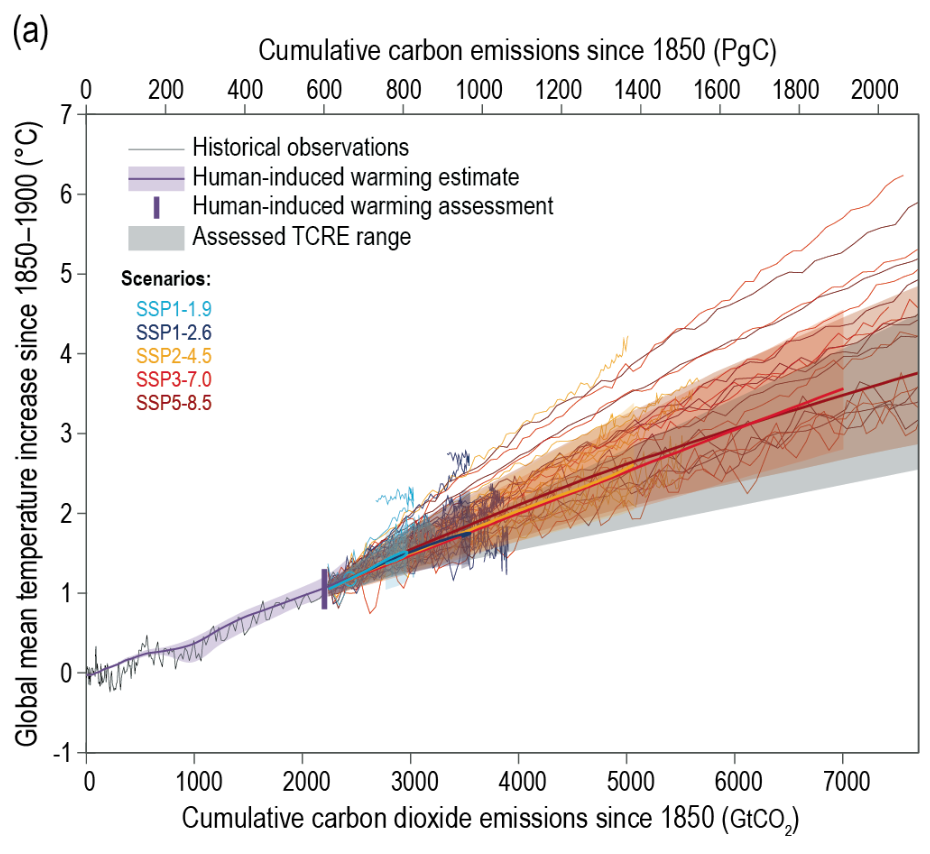
\includegraphics[width=0.2\linewidth]{tax/TCRS.png}\\
{\scriptsize Figure from IPCC 6.}
\end{center}
\column{0.44\textwidth}
\textbf{Damages: stochastic climate tipping.}
\begin{itemize}\itemsep2pt
    \item Damages reduce output; stochastic tipping as in \cite{weitzman2012ghg,kotlikoffParetoimprovingCarbonriskTaxation2021a}: irreversible damage to the environment (e.g., \citealp{lenton2008tipping}).
    \item Damage function:
    \begin{equation}
        \label{eq:damage_func_tipping}
    \Omega_t \left( T_{ t} \right) =  \frac{1}{1 + \left(\frac{1}{\psi_1} T_{ t} \right)^{2} + \left( \frac{1}{2 \cdot TP_{t}} T_{ t} \right)^{6.754}}
    \end{equation}
    where $\psi_1$ is a damage parameter and $TP_t$ follows a random walk truncated at $TP_t \in [2.5, 3.5]$.
    \item Once the temperature hits a tipping point, $TP_t$ stays at the given level.
    \item Shock processes for $\kappa_t$ and $TP_t$: appendix.
\end{itemize}
\end{columns}
\end{frame}

% == F31 [TAX: Equilibrium Conditions] ==
\begin{frame}[fragile]{Equilibrium Conditions}
{\footnotesize This system defines the DEQN loss for today's application.}
\begin{footnotesize}
  \begin{columns}[t]
        \begin{column}{0.5\textwidth}
        \textbf{Firm:}
            \begin{align}
                0 & = \tau_t \kappa_t  - \Omega_t (T_{\mathrm{AT}, t}) \theta_1 \theta_2 \mu_t^{\theta_2 -1} \tag{$\mu_t$}\\
                r_t & = \left( \Omega_t (T_{\mathrm{AT}, t}) (1 - \theta_1 \mu_t^{\theta_2}) \right. \notag \\
                    & \quad \left. - \tau_t \kappa_t (1 - \mu_t) \right) \alpha K_t^{\alpha - 1} L_t^{1 - \alpha} - \delta \tag{$K_t$}\\
                w_t & = \left( \Omega_t (T_{\mathrm{AT}, t}) (1 - \theta_1 \mu_t^{\theta_2}) \right. \notag\\
                    & \quad \left. - \tau_t \kappa_t (1 - \mu_t) \right) (1 - \alpha) K_t^{\alpha} L_t^{-\alpha} \tag{$L_t$}
            \end{align}
            \textbf{Households:}

            For all households $j \in 1,...,A-1$:
            \begin{align}
                c_t^{-\sigma}  = \beta \mathbb{E}_t \left[ (1+ r_{t+1}) c_{t+1,j+1}^{-\sigma} \right] \tag{EE} \\
                C_{t,j} + a_{t+1, j+1}  =  (1 + r_t) a_{t,j} + w_{t} l_{t,j} + \mathbb{T}_{t,j}  \tag{BC}
            \end{align}
            and initial/final conditions $a_{t,1} = 0$, $a_{t+1,A} = 0$.
        \end{column}
        \begin{column}{0.5\textwidth}
            \textbf{Market Clearing:}
            \begin{align}
                K_t & = \sum_{j = 1}^{A} a_{t,j} \tag{$K_t$}\\
            L_t & = \sum_{j = 1}^{A} l_j \tag{$L_t$} \\
            \tau_{t} e_t & = \sum_{j=1}^{A} \mathbb{T}_{t,j}  \tag{$\mathbb{T}$}
            \end{align}
        \end{column}
  \end{columns}
\end{footnotesize}
\end{frame}

% == F32 [TAX: The Planner's Problem] ==
\begin{frame}[fragile]{The Planner's Problem}
\small
\begin{itemize}
    \setlength\itemsep{0.8em}
    \item \textbf{Objective:} The planner chooses policy parameters $\vartheta$ (taxes \& transfers) to maximize the Social Welfare Function $\mathcal{W}$:
    \begin{align}
       \max_{\vartheta} \quad & \mathcal{W}(\vartheta) = \sum_{t = -10}^{30} \gamma_t \tilde{U}_t(\vartheta) \\
       \text{s.t.} \quad & \tilde{U}_t(\vartheta) \ge U_t \quad \forall t \quad \text{(if Pareto constrained)} \nonumber
    \end{align}
    \vspace{-0.5em}
    {\footnotesize (Where $\tilde{U}_t(\vartheta)$ is the ex-ante expected lifetime utility of generation $t$)}
    \item \textbf{Welfare Metric:} Gains are reported as the consumption equivalence factor ($\text{CE}_t$):
    \[
       \text{CE}_t = \left(\frac{\tilde{U}_t}{U_t}\right)^{\frac{1}{1-\sigma}}-1 \quad \text{\small{(where $U_t$ is BAU utility)}}
    \]
    \item \textbf{Scope \& Challenge:}
    \begin{itemize}
        \item Horizon: 40 generations (11 current, 29 future).
        \item Complexity: Solving for the optimal high-dimensional vector $\vartheta$ in a stochastic setting.
    \end{itemize}
\end{itemize}
\end{frame}

% == F33 [TAX: Mapping the OLG Model to DEQN], trimmed ==
\begin{frame}[fragile]{Mapping the OLG Model to DEQN}
\noindent\textbf{Goal:} Approximate the policy functions of the OLG model using a neural network: the $(z, K, \varrho) \rightarrow s$ network of Session 2, scaled up.

\vspace{0.4cm}
\begin{columns}
\begin{column}{0.55\textwidth}
\textbf{Inputs (state vector):}
\[
x = \big[t,\; TP_t,\; TP_{\mathrm{reached}},\; \kappa_t,\; a_{t,j},\; E_t,\;
\textcolor{blue}{\vartheta}\big]
\in \mathbb{R}^{A + 5 + d_\vartheta}
\]
\textbf{Outputs (policy vector):}
\[
y = \big[a_{t+1,j+1},\; v_{t,j}\big]
\in \mathbb{R}^{2(A-1)}
\]
\textbf{Policy map:}
\[
\Pi: x \;\Rightarrow\; y
\]
\end{column}
\begin{column}{0.42\textwidth}
\textbf{Pseudo-states $\boldsymbol{\vartheta}$:}
\begin{itemize}
  \item $d_\vartheta = 16$: 4 tax parameters + 12 transfer shares.
  \item \textcolor{blue}{DEQN learns policies for all tax rules and transfers at once}.
\end{itemize}
\vspace{0.3cm}
\textbf{Performance:}
\begin{itemize}
  \item Runtime from scratch: $\approx$4h on laptop.
  \item Warm start: a few minutes.
  \item Accuracy: MSE $\sim 10^{-6}$,\newline
  EE $\sim 10^{-3}$.
\end{itemize}
\end{column}
\end{columns}
\end{frame}

% == F34 [TAX: Approximating Welfare with Surrogates] ==
\begin{frame}{Approximating Welfare with Surrogates}
\small
    \textbf{The Computational Bottleneck:}
    \begin{itemize}
        \item DEQN solves the equilibrium, but evaluating expected welfare $\mathbb{E}[\mathcal{W}]$ requires expensive Monte Carlo simulations (10,000 paths per policy $\vartheta$).
        \item \textbf{Solution:} Train a \textcolor{blue}{Gaussian Process (GP)} to map policy parameters $\vartheta$ directly to welfare outcomes.
    \end{itemize}
    \vspace{0.1em}
    \textbf{Two Optimization Targets (QoIs):}
    \begin{columns}[t]
        \begin{column}{0.48\textwidth}
            \begin{block}{1. Maximize Aggregate Welfare}
                \small
                \textbf{Goal:} Maximize scalar $\mathcal{W}$.
                \[ \max_\vartheta \mathbb{E}_0[\mathcal{W}(\vartheta)] \]
                \begin{itemize}
                    \item \textbf{Surrogate:} Single scalar GP.
                    \item \textbf{Implication:} Ignores distribution (allows losers).
                \end{itemize}
            \end{block}
        \end{column}
        \begin{column}{0.48\textwidth}
            \begin{block}{2. Pareto Improvement}
                \small
                \textbf{Goal:} Maximize $\mathcal{W}$ subject to:
                \[ \tilde{U}_t(\vartheta) \ge U_t \quad \forall t \]
                \begin{itemize}
                    \item \textbf{Surrogate:} Vector of 40 GPs (one per cohort).
                    \item \textbf{Implication:} No generation is worse off.
                \end{itemize}
            \end{block}
        \end{column}
    \end{columns}
\end{frame}

% == F35 [TAX: The Engine: Gaussian Processes & Active Learning] ==
\begin{frame}{The Engine: Gaussian Processes \& Active Learning}
    \begin{columns}[t]
        \begin{column}{0.45\textwidth}
            \centering
            \textbf{1. Gaussian Processes (GP)}
            \vspace{0.3em}

            \resizebox{0.72\textwidth}{!}{
            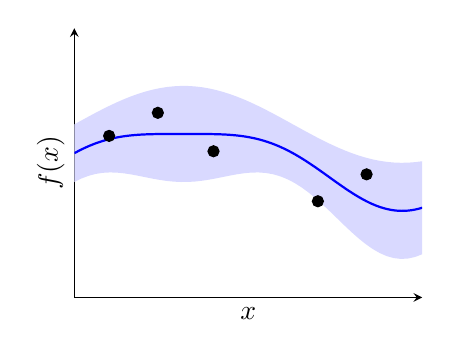
\begin{tikzpicture}
                \begin{axis}[
                    xlabel={$x$}, ylabel={$f(x)$},
                    ticks=none, axis lines=left,
                    ymin=-3, ymax=4, xmin=0, xmax=5,
                    height=5cm, width=6cm
                ]
                    \addplot[name path=A, draw=none, domain=0:5, samples=50] {sin(deg(x)) + 1.5};
                    \addplot[name path=B, draw=none, domain=0:5, samples=50] {sin(deg(x)) - 0.5 + 0.5*cos(deg(x)*2)};
                    \addplot[fill=blue!15, draw=none, forget plot] fill between[of=A and B];
                    \addplot[blue, thick, domain=0:5, samples=100] {sin(deg(x)) + 0.5 + 0.25*cos(deg(x)*2)};
                    \addplot[only marks, mark=*, mark size=2pt] coordinates {(0.5, 1.2) (1.2, 1.8) (2.0, 0.8) (3.5, -0.5) (4.2, 0.2)};
                \end{axis}
            \end{tikzpicture}
            }

            \vspace{0.2em}
            \scriptsize{
            Kernel:
            \[
            k(x, x') = \sigma_f^2 \exp\!\left(-\frac{\|x - x'\|^2}{2\ell^2}\right)
            \]
            Predictive mean \& variance:
            \begin{align*}
            \mu(x^*) &= k_*^\top (K + \sigma_n^2 I)^{-1} \mathbf{y} \\
            \sigma^2(x^*) &= k(x^*, x^*) - k_*^\top (K + \sigma_n^2 I)^{-1} k_*
            \end{align*}
            }
        \end{column}
        \begin{column}{0.55\textwidth}
            \centering
            \textbf{2. Bayesian Active Learning (BAL)}

            \vspace{0.2em}
            \small{
            \[ \alpha(x) = \underbrace{\mu(x)}_{\text{Exploit}} + \kappa \cdot \underbrace{\sigma(x)}_{\text{Explore}} \]
            }

            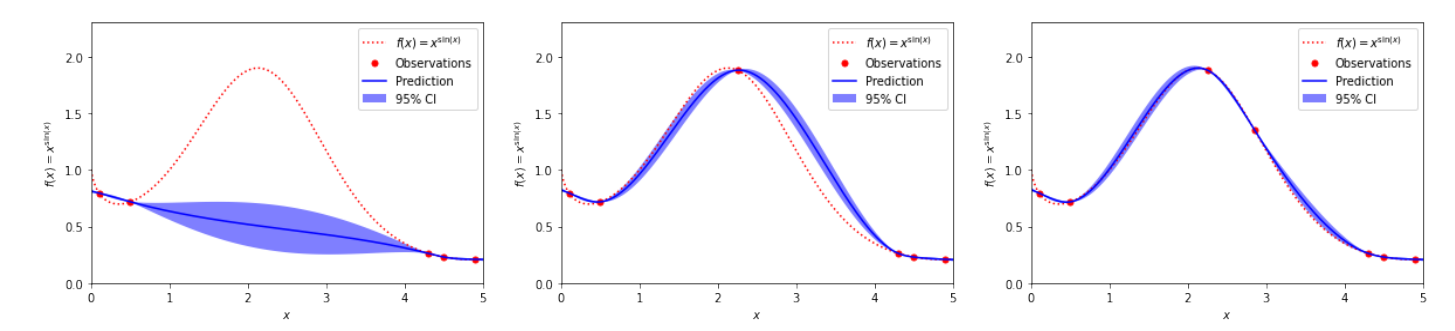
\includegraphics[width=0.82\linewidth, keepaspectratio]{tax/bal.png}

            \vspace{0.3em}
            \footnotesize{\textit{We simulate points that maximize this score, reducing computational cost by orders of magnitude.}}
        \end{column}
    \end{columns}
\end{frame}

% == F36 [TAX: Constructing the Welfare Surrogate] ==
\begin{frame}{Constructing the Welfare Surrogate}
    \begin{columns}[t]
        \begin{column}{0.32\textwidth}
            \begin{block}{1. The Mapping}
                \small
                We map policy rules directly to \textbf{Expected Welfare}:
                \[
                    \vartheta \longmapsto \mathbb{E}_0[\mathcal{W}(\vartheta)]
                \]
                \begin{itemize}
                    \item \textbf{Input ($\vartheta$):} Tax and transfer parameters.
                    \item \textbf{Target:} Monte Carlo mean of lifetime utilities.
                \end{itemize}
            \end{block}
        \end{column}
        \begin{column}{0.32\textwidth}
            \begin{block}{2. Active Training}
                \small
                We populate the training set $\mathcal{D}$ efficiently:
                \begin{itemize}
                    \item \textbf{Initial Design:} 450 points sampled randomly (Latin Hypercube).
                    \item \textbf{Refinement:} 50 points added via \textcolor{blue}{Bayesian Active Learning (BAL)}.
                    \item \textbf{Total:} Only 500 simulations needed.
                \end{itemize}
            \end{block}
        \end{column}
        \begin{column}{0.32\textwidth}
            \begin{block}{3. The Model}
                \small
                Fitting the Gaussian Process:
                \begin{itemize}
                    \item \textbf{Kernel:} Squared Exponential with Automatic Relevance Detection (ARD).
                    \item \textbf{Accuracy:} Leave-One-Out (LOO) error $\approx \mathbf{10^{-4}}$.
                    \item \textbf{Result:} A smooth, cheap-to-query surface.
                \end{itemize}
            \end{block}
        \end{column}
    \end{columns}

\vspace{0.2em}
{\footnotesize \emph{Robustness.} Training is anchored on a handful of trusted reference solutions to avoid \emph{lazy learning} --- the flat-in-the-parameter failure mode discussed in Session 1; 10--20 anchors suffice \citep{friedlDeep2023}.}
\end{frame}

% == F37 [TAX: Maximizing Welfare] + mandatory callback (b) ==
\begin{frame}{Maximizing Welfare}
\begin{itemize}
    \item We now have a cheap-to-evaluate surrogate model to map \textcolor{blue}{tax functions onto welfare}. But we still need to find the optimal tax.
    \vspace{0.3cm}
    \item We aim to \textcolor{blue}{find the $\argmax$ of our surrogate model}, which gives us the optimal tax function parameters:
    \[
       \vartheta^* = \argmax_{\vartheta} \widehat{\mathrm{QoI}}(\vartheta)
    \]
    s.t. various constraints.
    \vspace{0.3cm}
    \item We use \textcolor{blue}{constrained optimization with linear constraints} for periods \{0,T\} that ensure that the parameters of the tax function stay within the feasible range during optimization.
    \end{itemize}
\vspace{0.3cm}
\begin{block}{Callback to Session 2}
Same object as the SMM criterion, opposite sign of intent: there we minimized distance to data, here we maximize welfare.
\end{block}
\end{frame}

% == F38 [TAX: Three Policy Scenarios] ==
\begin{frame}{Three Policy Scenarios}
\small
    \begin{itemize}
        \setlength\itemsep{1em}
        \item \textbf{Scenario 1: Unconstrained Welfare Maximization} \\
        \small{Linear tax on cumulative emissions + exogenous transfers.}
        \begin{equation*}
            \tau_t(E_t) = \vartheta_0 + \vartheta_E \cdot E_t
        \end{equation*}
        \item \textbf{Scenario 2: Pareto-Improving Policy} \\
        \small{Linear tax on cumulative emissions + \textbf{optimal} transfers.}
        \begin{equation*}
             \tau_t(E_t) = \vartheta_0 + \vartheta_E \cdot E_t
        \end{equation*}
        \item \textbf{Scenario 3: Increasing Policy Complexity} \\
        \small{Linear tax on cumulative emissions, carbon intensity ($\kappa$), and tipping risk ($TP$) + optimal transfers.}
        \begin{equation*}
            \tau_t(\cdot) = \vartheta_0 + \vartheta_E E_t + \vartheta_\kappa \kappa_t + \vartheta_{TP} (1-\mathbb{D}_{TP})
        \end{equation*}
    \end{itemize}
\end{frame}

% == F39 [TAX: Scenario 1], absorbing Redistribution of Tax Income ==
\begin{frame}{Scenario 1: Unconstrained Welfare Maximization}
\small
Each period's tax income is redistributed to currently alive agents; in general, \textcolor{blue}{transfer schemes may create winners and losers} \citep{kotlikoff2021making}. Here: the ``10\% scheme''. The youngest generation receives the largest share of total tax revenue, and the share for each older generation decreases by 10\% relative to the next younger one. The shares are normalized to sum to one. Formally, our transfer scheme, $\mathbb{T}$, is defined as:
\begin{equation}
    \mathbb{T}_{t,j} = 0.9^{(j-1)} \cdot 0.1394 \cdot \tau_t e_t, \quad j \in \{2,...,12 \}.
\end{equation}
The resulting constrained optimization problem reads as:
\begin{equation}
\label{eq:optim_cum_emm_maxwelf}
\begin{aligned}
  \vartheta^{\ast}
  \;=\;
  & \arg\max_{\vartheta\in[a,b]}\,
  \widehat{\mathrm{QoI}}(\vartheta) \\
& \quad \text{s.t.} \\
& 0 \leq \vartheta_0 + \vartheta_E  E_0 \leq \bar{\tau}, \\
& 0 \leq \vartheta_0 + \vartheta_E  E_{29} \leq \bar{\tau}.
\end{aligned}
\end{equation}
\end{frame}

% == F40 [TAX: The Welfare Surrogate (Scenario 1)] ==
\begin{frame}{The Welfare Surrogate (Scenario 1)}
\begin{columns}[c]
    \begin{column}{0.55\textwidth}
        \centering
        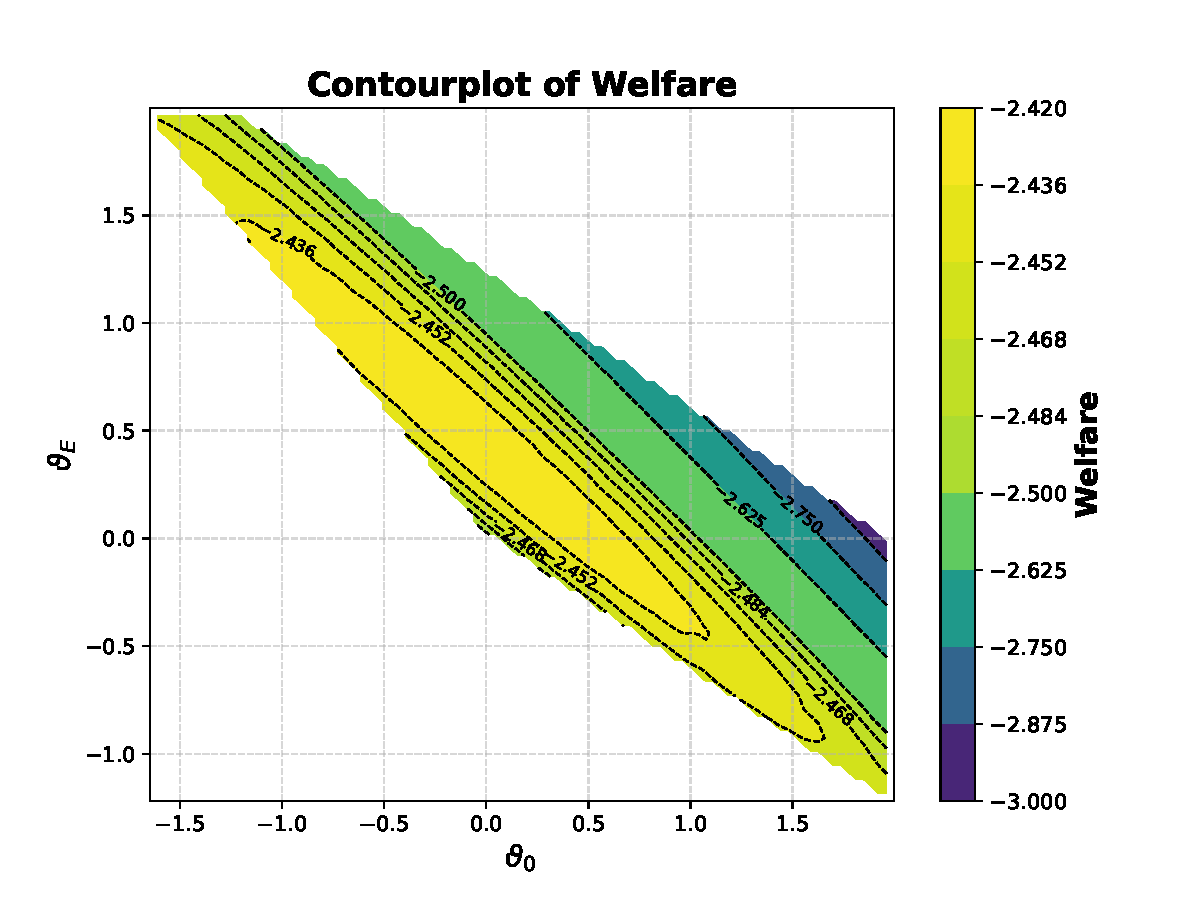
\includegraphics[width=0.92\linewidth]{tax/paper/contour_welfare_E.pdf}
    \end{column}
    \begin{column}{0.42\textwidth}
        \small
        \begin{itemize}
            \setlength\itemsep{1em}
            \item \textbf{The Surface:} A Gaussian Process approximation of the Social Welfare Function.
            \item \textbf{The Axes:} Tax Intercept ($\vartheta_0$) vs. Slope ($\vartheta_E$).
            \item \textbf{The Goal:} Find the ``peak'' (yellow zone) without running millions of simulations.
            \item \textbf{Precision:} Leave-One-Out error $\approx \mathbf{10^{-5}}$.
        \end{itemize}
    \end{column}
\end{columns}
\end{frame}

% == F41 [TAX: Optimal Welfare Distribution] ==
\begin{frame}{Optimal Welfare Distribution}
\begin{columns}[c]
    \begin{column}{0.55\textwidth}
        \centering
        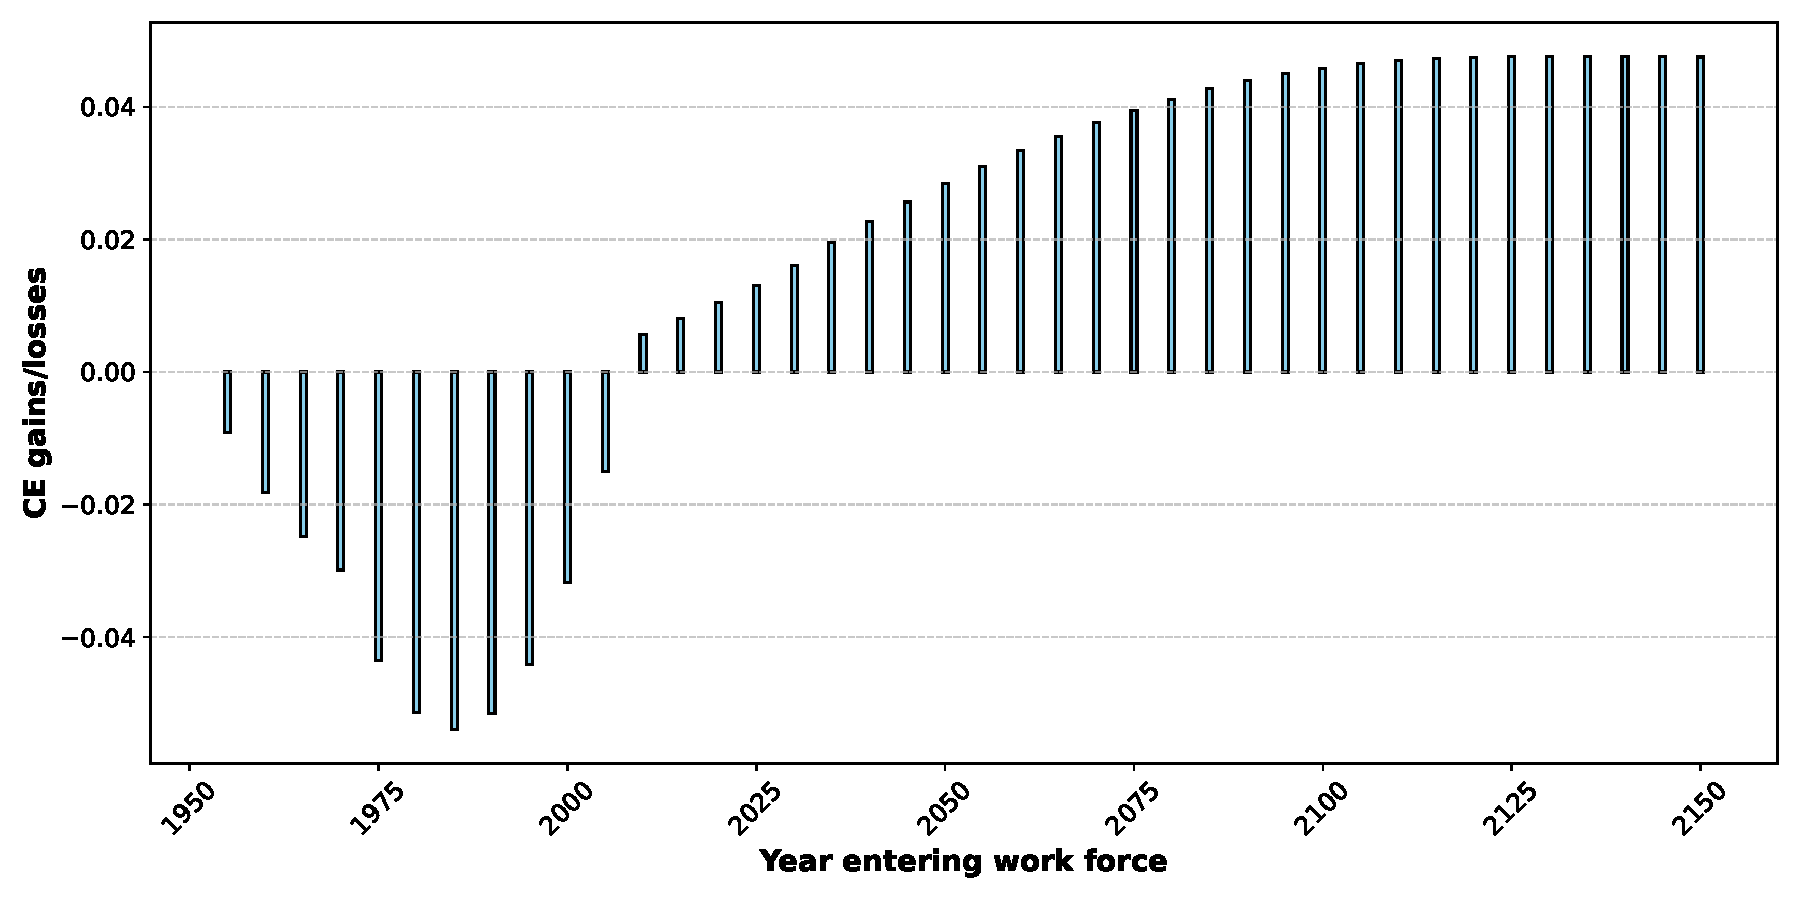
\includegraphics[width=0.92\linewidth]{tax/paper/lin_S_10trans_unif_welfares.pdf}
    \end{column}
    \begin{column}{0.42\textwidth}
        \small
        \textbf{The Price:}
        \begin{itemize}
            \setlength\itemsep{0.8em}
            \item \textbf{Aggregate Welfare Gain:} The total pie grows by \textbf{1.6\%} (consumption equivalent).
            \item \textbf{Future Gain:} Generations born after 2100 enjoy gains of $\approx \mathbf{4.8\%}$.
            \item \textbf{Current Pain:} \textcolor{red}{This comes at a steep cost.} Transition generations suffer losses up to \textbf{5\%}.
            \item \textbf{Conclusion:} Without transfers, this optimal policy is politically dead on arrival.
        \end{itemize}
    \end{column}
\end{columns}
\end{frame}

% == F42 [NEW, merge: TAX The Challenge (lead-in) + Scenario 2: Pareto-Improving Policy] ==
\begin{frame}{Scenario 2: Pareto-Improving Policy}
\footnotesize
Lead-in: the welfare-maximizing tax reduces warming to $2.7^\circ$C, \textbf{but} imposes welfare losses of up to \textbf{5\%} on current older generations: economically efficient, politically infeasible. \textbf{Goal:} a tax \textit{and} transfer scheme where $\tilde{U}_t \ge U_t$ for all $t$.

\vspace{0.2em}
For 40 values of $t$:
\begin{equation}
    \mu_{*,t}(\vartheta) \;=\; \widehat{\mathrm{QoI}}_t(\vartheta)
  \;=\;
  \mathbb{E}\!\bigl[\tilde{U}_t(\vartheta)\bigr] \quad \forall \; t \in \{-10,...,29\}
\end{equation}
Solve:
\begin{equation}
\label{eq:opt_pareto_y2}
\begin{aligned}
  &\vartheta^{\ast}
  \;=\;
  \arg\max_{\vartheta\in[a,b]}
  \sum_{t=-10}^{29}\gamma_t\, \widehat{\mathrm{QoI}}_t(\vartheta)
  \;=\;
  \arg\max_{\vartheta\in[a,b]}
  \sum_{t=-10}^{29}\gamma_t\,\mathbb{E}_0\!\bigl[\tilde{U}_t(\vartheta)\bigr] \\
& \quad \text{s.t.} \quad
 \mathbb{E}_0\!\bigl[\tilde{U}_t(\vartheta)\bigr]
  \;\ge\;
  \mathbb{E}_0\!\bigl[U_t\bigr]
  \;\;\forall\,t, \\
& \phantom{\quad \text{s.t.} \quad} 0 \leq \vartheta_0 + \vartheta_E  E_0 \leq \Bar{\tau}, \qquad
 0 \leq \vartheta_0 + \vartheta_E  E_{29} \leq \Bar{\tau},  \qquad
 \sum_{i=1}^{12} \vartheta_i = 1
\end{aligned}
\end{equation}
\end{frame}

% == F43 [TAX: Optimal Parameters and Transfers] ==
\begin{frame}{Optimal Parameters and Transfers}
We find optimal tax parameters: $\vartheta_0 = -0.186$ and $\vartheta_E = 0.225$.\newline

The optimal transfer shares allocate resources to specific cohorts to satisfy the Pareto constraints:
\begin{table}[htbp]
\begin{small}
        \centering
    \begin{tabular}{|c|c|c|c|c|c|c|c|c|c|c|c|c|}
        \hline
        \textbf{t1} & \textbf{t2} & \textbf{t3} & \textbf{t4} & \textbf{t5} & \textbf{t6} & \textbf{t7} & \textbf{t8} & \textbf{t9} & \textbf{t10} & \textbf{t11} & \textbf{t12} \\
        \hline
        0.128 & 0.051 & 0.058 & 0.09 & 0.15 & 0.09 & 0.066 & 0.143 & 0.076 & 0.048 & 0.039 & 0.06 \\
        \hline
    \end{tabular}
    \caption{\textbf{Pareto optimal transfer scheme.} Optimal shares for each concurrent cohort $i$ under the linear cumulative emissions tax.}
    \label{tab:optimal_transfer_lin_S}
    \end{small}
\end{table}
\end{frame}

% == F44 [TAX: Optimal Welfare (Pareto Improving)] ==
\begin{frame}{Optimal Welfare (Pareto Improving)}
\begin{columns}[c]
    \begin{column}{0.55\textwidth}
        \centering
        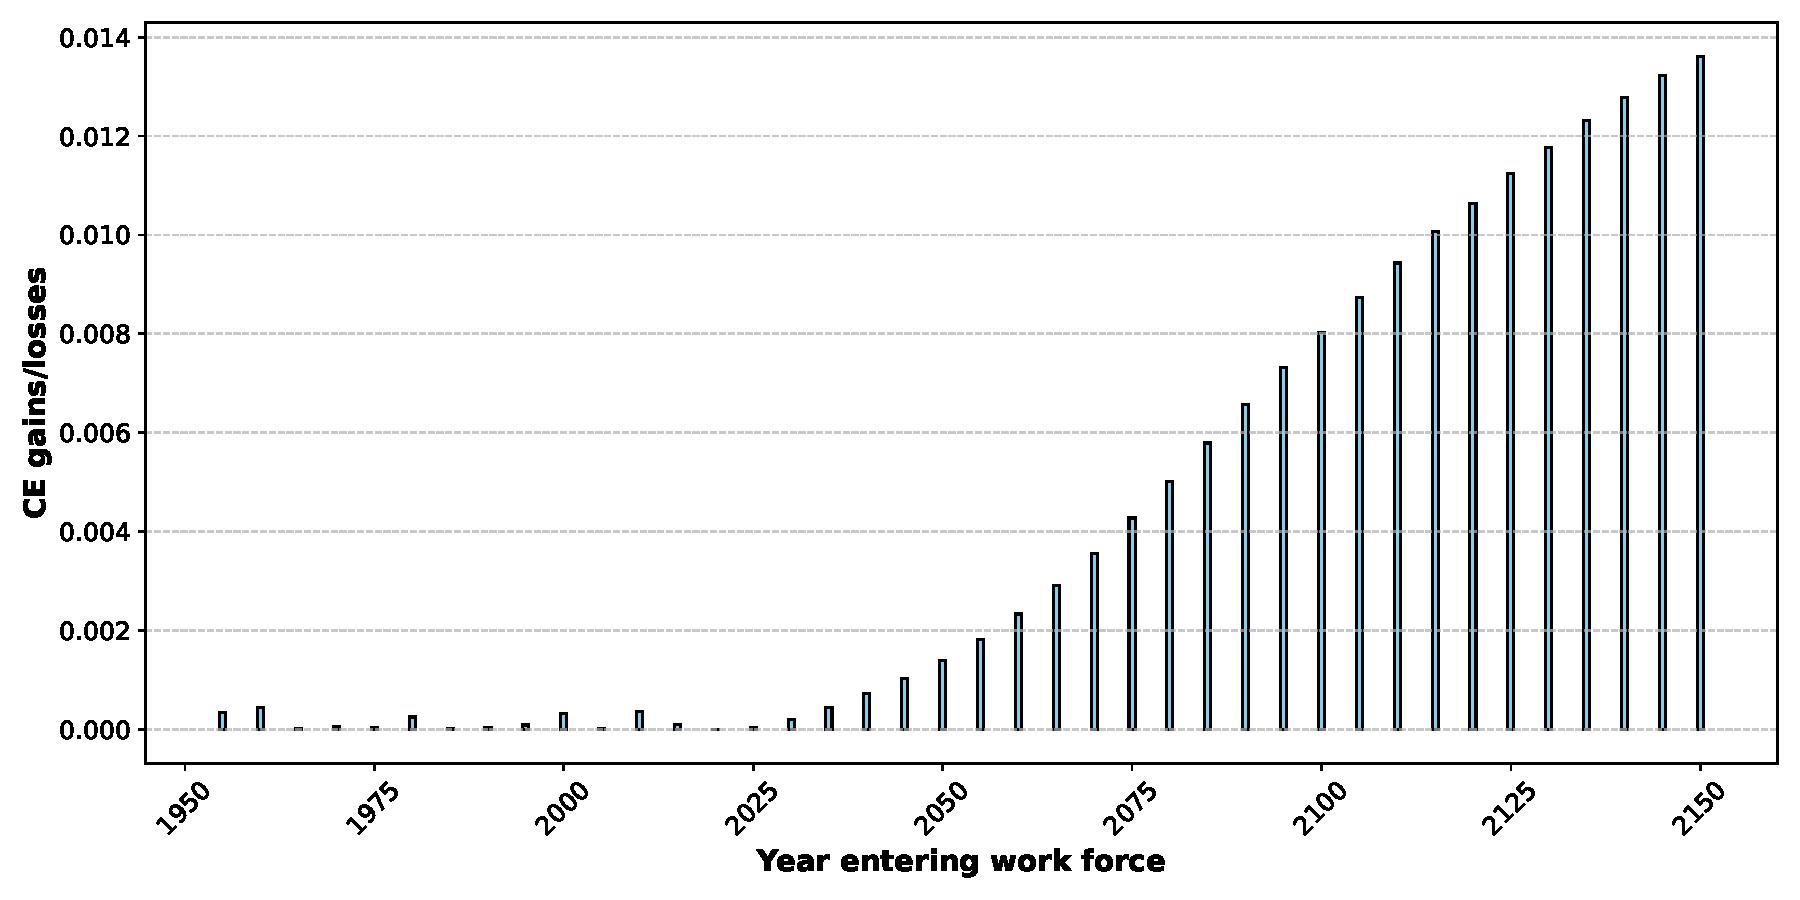
\includegraphics[width=0.92\linewidth]{tax/paper/welfare_gains_lin_S_trans.pdf}
    \end{column}
    \begin{column}{0.42\textwidth}
        \small
        \begin{itemize}
            \setlength\itemsep{0.8em}
            \item \textbf{The Pareto Constraint:} Transfers are explicitly optimized to keep initial generations (and those born in the next decade) at \textbf{BAU levels} (0\% loss).
            \item \textbf{Future Gains:} Welfare improves monotonically, reaching \textbf{$\approx$1.4\%} for distant generations.
            \item \textbf{The Cost of Consensus:} Compared to the unconstrained case (max 4.8\%), future gains are smaller, but \textbf{no generation loses}.
            \item \textbf{Aggregate:} Total welfare gain of \textbf{0.42\%}.
        \end{itemize}
    \end{column}
\end{columns}
\end{frame}

% == F45 [TAX: Temperature (Scenario 2)], absorbing the insurance bullet ==
\begin{frame}{Temperature (Scenario 2: Pareto-Improving)}
\begin{columns}[c]
    \begin{column}{0.5\textwidth}
        \centering
        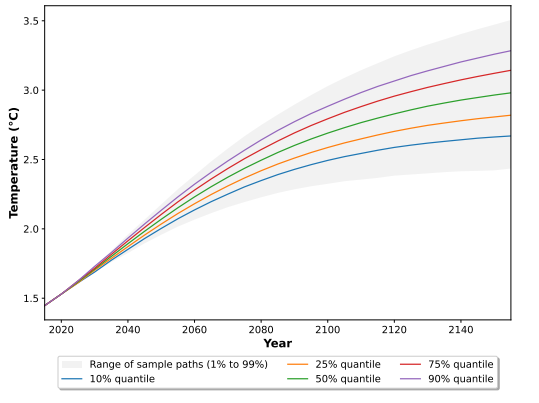
\includegraphics[width=0.92\linewidth]{tax/Temp_case2.png}
    \end{column}
    \begin{column}{0.47\textwidth}
        \small
        \begin{itemize}
            \setlength\itemsep{0.7em}
            \item \textbf{The Trade-off:} Mean warming settles just below \textbf{3\,°C} (higher than Scenario 1).
            \item \textbf{Crucial Insurance:} The 99th percentile \textbf{never exceeds 3.5\,°C}.
            \item \textbf{Tail Truncation:} The policy deliberately eliminates the catastrophic tail ($>$3.6\,°C under BAU).
            \item \textbf{The Win:} Achieved with optimal transfers $\to$ \textbf{no generation loses}.
            \item \textcolor{uzhblue}{\textbf{Conclusion:} The Pareto-optimal policy functions primarily as disaster insurance rather than aggressive mitigation.} {\footnotesize (Emissions distribution: appendix.)}
        \end{itemize}
    \end{column}
\end{columns}
\end{frame}

% == F46 [TAX: Scenario 3: Increasing Policy Complexity] ==
\begin{frame}{Scenario 3: Increasing Policy Complexity}
\small
    \textbf{Question:} Can we improve welfare by targeting specific climate drivers?
    \vspace{0.5em}

    We expand the tax rule to include \textbf{Carbon Intensity} ($\kappa_t$) and \textbf{Tipping Risk} ($TP_t$):
    \begin{equation}
        \label{eq:tax_fun_lin_S_kappa_tipping}
        \tau_t = \vartheta_0 + \vartheta_E \frac{E_t}{E_0} + \underbrace{\vartheta_\kappa \frac{\kappa_t}{\kappa_0}}_{\text{Intensity}} + \underbrace{\vartheta_{TP} (1 - \mathbb{D}_{TP})}_{\text{Tipping Risk}}
    \end{equation}
    \begin{itemize}
        \item $\mathbb{D}_{TP} \in [0,1]$: Normalized distance to the tipping threshold.
        \item \textbf{Dimensionality:} This adds new pseudo-states, increasing the parameter space to $d_\vartheta = 16$ (4 tax parameters + 12 transfer shares).
        \item We use the same ML-based optimization to find the constrained Pareto-optimal policy.
    \end{itemize}
\end{frame}

% == F47 [TAX: Results: Diminishing Returns to Complexity] ==
\begin{frame}{Results: Diminishing Returns to Complexity}
\small
    We find the optimal parameters:
    \[
        \{\vartheta_0, \vartheta_E, \vartheta_\kappa, \vartheta_{TP} \} = \{-0.237,\;  0.203, \;  0.037, \;  0.012 \}
    \]
    \textbf{Key Finding:} Complexity adds very little welfare value.
    \begin{table}[h]
        \centering
        \begin{tabular}{lcc}
            \toprule
            \textbf{Policy Specification} & \textbf{Instruments} & \textbf{Welfare Gain*} \\
            \midrule
            Linear in Cumulative Emissions ($E_t$) & 2 & \textbf{0.42\%} \\
            Linear in $E_t, \kappa_t, TP_t$ & 4 & \textbf{0.45\%} \\
            \bottomrule
        \end{tabular}
        \caption{\footnotesize Aggregate welfare gains in consumption-equivalent terms.}
    \end{table}
    \begin{alertblock}{Conclusion:}
        A simple, well-designed tax on cumulative emissions captures \textbf{93\%} of the potential welfare gains. Adding complex state-dependencies provides only marginal benefits.
    \end{alertblock}
\end{frame}

% == F48 [TAX: The Cost of Political Feasibility] ==
\begin{frame}{The Cost of Political Feasibility}
\small
    Comparing the physical outcomes of the two approaches reveals a crucial trade-off: \newline
    \begin{columns}[t]
        \begin{column}{0.5\textwidth}
            \textbf{1. Welfare Maximizing} \\ (Unconstrained)
            \begin{itemize}
                \item \textcolor{blue}{Aggressive early mitigation.}
                \item Warming stabilizes at $\mathbf{\approx 2.7^\circ C}$.
                \item \textcolor{red}{Current generations lose (up to 5\%).}
            \end{itemize}
        \end{column}
        \begin{column}{0.5\textwidth}
            \textbf{2. Pareto Improving} \\ (Constrained)
            \begin{itemize}
                \item \textcolor{blue}{Slower initial mitigation path.}
                \item Warming stabilizes at $\mathbf{\approx 3.0^\circ C}$.
                \item \textcolor{green}{No generation loses.}
                \item \textbf{\textcolor{uzhorange}{Crucial: Truncates worst-case damages (insurance).}}
            \end{itemize}
        \end{column}
    \end{columns}
    \vspace{0.8em}
    \begin{alertblock}{Trade-off \& Insurance}
        Ensuring political support requires delaying some mitigation, leading to higher \textit{average} temperatures ($\approx +0.3^\circ C$). However, it successfully \textbf{eliminates extreme damage scenarios} ($>15\%$ of GDP), effectively insuring future generations against climate disasters.
    \end{alertblock}
\end{frame}

% =====================================================================
% Section 5: Synthesis and conclusion
% =====================================================================
% TIMING: cumulative 78 min when this section starts
\section{Synthesis}

% == F49 [NEW]: three-column synthesis table ==
\begin{frame}{One Surrogate, Three Questions}
\scriptsize
\begin{center}
\begin{tabular}{p{0.13\textwidth}p{0.24\textwidth}p{0.25\textwidth}p{0.24\textwidth}}
\toprule
 & \textbf{Session 2: SMM} & \textbf{Appendix: UQ} & \textbf{Today: Design} \\
\midrule
Model & Brock--Mirman & stochastic IAM with Bayesian learning about the ECS & stochastic OLG IAM with tipping risk \\
Surrogate inputs & $(z, K, \beta, \varrho)$ & climate-economy states plus uncertain $\bm{\theta}$ (9+N states) & OLG IAM state plus 16 policy pseudo-states \\
QoI & moments $m_1$ to $m_3$ & $\mathrm{SCC}(\theta_1,\dots,\theta_N)$ & 40 cohort welfares \\
Second surrogate & none needed & GP + Bayesian active learning & GP $\times 40$ with BAL \\
Operator & $\argmin$ under CRN & global sensitivity analysis (UE, Sobol', Shapley) & constrained $\argmax$ \\
Output & interior estimate & importance ranking of parameters & Pareto-improving tax \\
Headline & identification-ridge lesson & ECS and damage-function uncertainty drive the SCC & 0.42\% aggregate gain \\
\bottomrule
\end{tabular}
\end{center}
\end{frame}

% == F50 [NEW]: practical guidance, sourced only ==
\begin{frame}{Practical Guidance}
\small
\begin{itemize}\itemsep6pt
\item \textbf{Train once, then simulate for free.} Surrogate 1 costs about 4h from scratch on a laptop, a few minutes warm-started; once trained, the solution allows us to simulate data essentially for free.
\item \textbf{When the second surrogate pays off.} Whenever a single QoI point is expensive: expected welfare needs 10{,}000 Monte Carlo paths per policy $\vartheta$; the GP + BAL layer reduces this to 500 simulations total (450 Latin hypercube + 50 actively learned), at LOO error $\approx 10^{-4}$.
\item \textbf{A generic blueprint.} A universal framework for \textbf{almost any} stochastic heterogeneous-agent model: it allows researchers to both \textcolor{blue}{solve global equilibria} and derive \textcolor{blue}{constrained-optimal policies} in settings previously deemed intractable.
\item \textbf{Production-scale reference.} Chen, Didisheim \& Scheidegger (2026, \emph{J.\ Financial Economics}): exactly this surrogate logic at scale, applied to finance.
\end{itemize}
\end{frame}

% == F51 [NEW]: extensions and open questions, sourced items only ==
\begin{frame}{Extensions and Open Questions}
\small
\textbf{Extensions on the authors' agenda:}
\begin{itemize}\itemsep2pt
\item Analyze richer, non-linear tax functions, solve for the optimal tax, and construct the Pareto frontier.
\item Optimal transfers in a ``quadratic'' (parametrized) tax model.
\item Based on high-dimensional model representation~\citep{eftekhari_2022}, determine the dominant terms that are driving the results.
\item Add multiple global regions to the model to study the distributional effects of climate change.
\end{itemize}
\vspace{0.5em}
\textbf{Open questions (bridges between the main part and the appendix; not in the source papers):}
\begin{itemize}\itemsep2pt
\item Apply the \emphc{quantify} operator to the \emphc{design} output: how sensitive is $\vartheta^*(\bm{\theta})$ to the structural parameters?
\item Propagate Session 2-style estimation uncertainty in $\hat{\bm{\theta}}$ into the SCC.
\end{itemize}
\end{frame}

% == F52 [TAX: Conclusion], rebuilt to span all three operators ==
\begin{frame}{Conclusion}
    \begin{columns}
        \begin{column}{0.62\textwidth}
            \small
            \begin{itemize}
                \setlength{\itemsep}{0.9em}
                \item \textbf{One pipeline, three operators:} \\
                A scalable ML framework (\textcolor{blue}{DEQN + GP + post-processing}) supports \emphc{estimate} (Session 2: SMM with an interior estimate), \emphc{quantify}, and \emphc{design} on the same trained surrogate.
                \item \textbf{Quantify (appendix):} \\
                Uncertainty in the SCC is mainly driven by parametric uncertainty in the ECS and the damage function.
                \item \textbf{Design (main part):} \\
                Simple linear tax + optimal transfers $\rightarrow$ \textbf{Pareto improvement}, with a \textbf{0.42\%} aggregate welfare gain; added complexity yields only marginal gains (to \textbf{0.45\%}): simple, implementable rules capture the vast majority of benefits.
                \item \emphc{Solve once, ask many questions.}
            \end{itemize}
        \end{column}
        \begin{column}{0.36\textwidth}
            \centering
            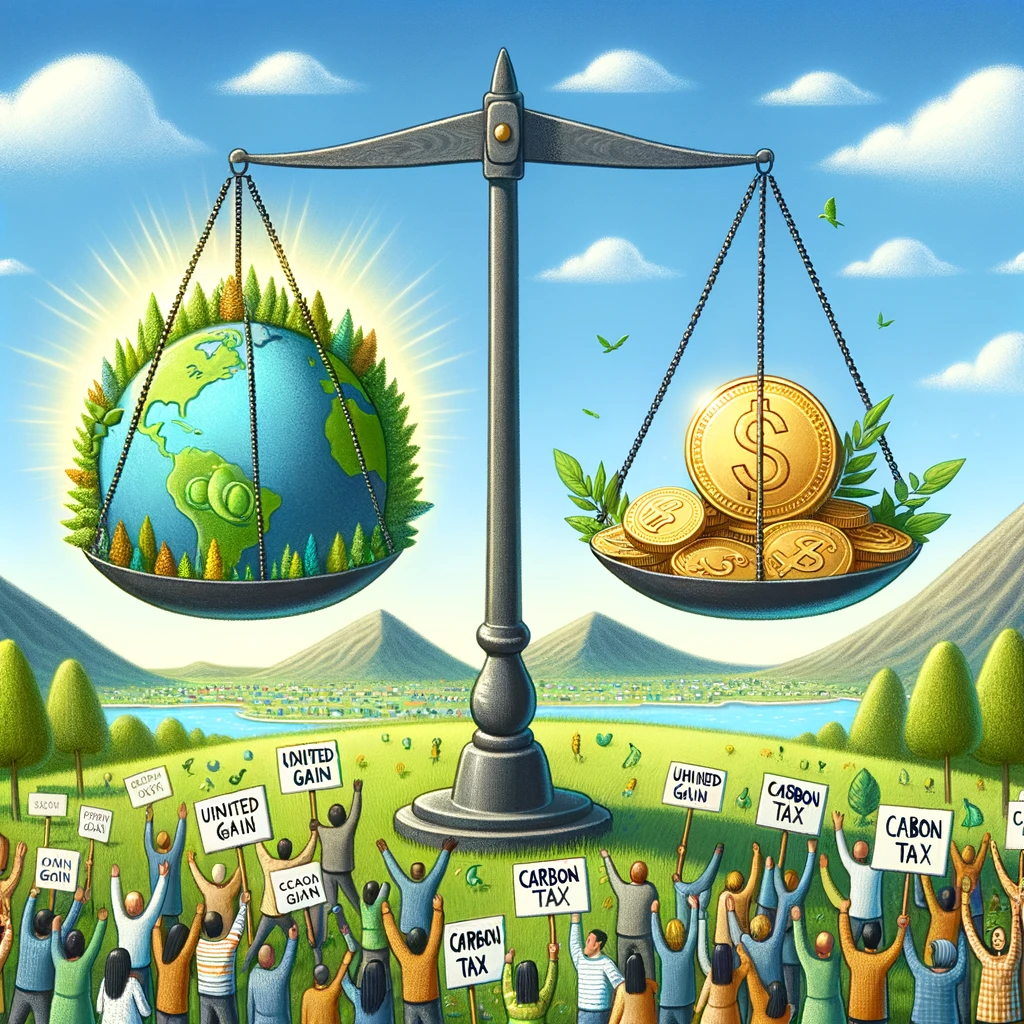
\includegraphics[width=0.9\linewidth]{tax/summary_happy.png}
        \end{column}
    \end{columns}
\end{frame}

% == F53 [TAX: Questions?], course styling ==
{\setbeamercolor{background canvas}{bg=uzhgreylight}
\begin{frame}
\Huge \textcolor{uzhorange}{Questions?}
\end{frame}}

% =====================================================================
% Appendix
% =====================================================================
\appendix
\backupbegin

% == A1 [TAX: What is a deep neural net?] ==
\begin{frame}
\frametitle{Appendix: What is a deep neural net?}
\begin{align*}
\textbf{input} := x &\rightarrow \textcolor{blue}{\phi^1(}W^1_{\bm{\rho}} x + \textbf{b}^1_{\bm{\rho}}\textcolor{blue}{)} =: \textbf{hidden 1}\\
\rightarrow\textbf{hidden 1} &\rightarrow \textcolor{blue}{\phi^2(}W^2_{\bm{\rho}} (\textbf{hidden 1}) + \textbf{b}^2_{\bm{\rho}}\textcolor{blue}{)} =:\textbf{hidden 2}\\
\rightarrow\textbf{hidden 2}&\rightarrow \textcolor{blue}{\phi^3(}W^3_{\bm{\rho}} (\textbf{hidden 2}) + \textbf{b}^3_{\bm{\rho}}\textcolor{blue}{)}=: \textbf{output}
\end{align*}
The neural net is then given by the choice of activation functions and the parameters ${\bm{\rho}}$.
\begin{figure}
    \centering
    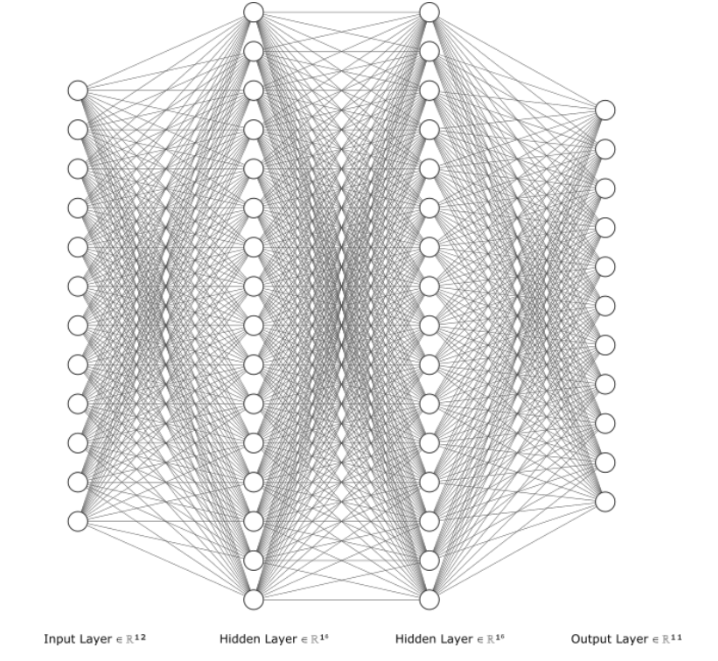
\includegraphics[width=0.3\textwidth]{tax/nn-example.png}
\end{figure}
\end{frame}

% == A2 [TAX: Our loss function] ==
\begin{frame}
\frametitle{Appendix: Our loss function}
As a loss function, we implement
\begin{equation*}
\ell_{\bm{\rho}}:= \frac{1}{N_{\text{path length}}}\sum_{x_i \text{ on sim. path}}\left(\textbf{G}(x_i, \mathcal{N}_{\bm{\rho}})\right)^2
\end{equation*}
where we use $\mathcal{N}_{\bm{\rho}}$ to simulate a path. $\textbf{G}$ is chosen, such that the true equilibrium policy $\textbf{f}(x)$ is defined by $\textbf{G}(x, \textbf{f})=0~\forall x$.
Therefore, there is \textcolor{blue}{no need for labels} to evaluate our loss function.
\end{frame}

% == A3 [TAX: Training Deep Equilibrium Nets] ==
\begin{frame}
\frametitle{Appendix: Training Deep Equilibrium Nets\footnote{Sample codes here:~\url{https://github.com/sischei/DeepEquilibriumNets.}}}
\begin{enumerate}
\item Simulate a sequence of states $\mathcal{D}_{\text{train}}^i\gets\{x^i_1, x^i_2, \dots ,x^i_T\}$  from the policy encoded by the network parameters $\bm{\rho}^i$.
\item Evaluate the errors of the equilibrium conditions on the newly generated set $\mathcal{D}_{\text{train}}$.
\item If the error statistics are not low enough:
\begin{enumerate}
\item Update the parameters of the neural network with a gradient descent step (or a variant):
  \begin{equation}
  \rho^{i+1}_{k}=\rho^{i}_{k} - \alpha_{\text{learn}} \frac{\partial \ell_{\mathcal{D}_{\text{train}}^i}(\bm{\rho}^{i})}{\partial \rho^i_{k}} \nonumber.
  \end{equation}
  \item Set new starting states for simulation: $x^{i+1}_0 = x^i_T$.
  \item Increase $i$ by one and go back to step 1.
\end{enumerate}
\end{enumerate}
\end{frame}

% == A4 [TAX: Architecture of the Deep Neural Network], math-in-tabular fixed ==
\begin{frame}[fragile]{Appendix: Architecture of the Deep Neural Network}
    \begin{table}[h]
    \centering
    \begin{tabular}{|c|c|}
    \hline
    \textbf{Hyperparameter} & \textbf{Value} \\
    \hline
    Optimizer (LR) & Adam (1e-5) \\
    Batch size & 64 \\
    NN hidden layers & 2 \\
    NN units & 256  \\
    activation function & GeLu \\
    N inputs & 12 + 5 + $\vartheta$ \\
    N outputs & $2\cdot(A-1) = 22$ \\
    N epochs per episode & 1 \\
    N sim episode length & 70 (each step is 5y) \\
    N\_batches & 512 \\
    \hline
    \end{tabular}
    \caption{Hyperparameters of neural network.}
    \label{tab:nn_arch}
\end{table}
\end{frame}

% == A5 [TAX: Gaussian Process Regression: Theory] ==
\begin{frame}{Appendix: Gaussian Process Regression: Theory}
  \begin{columns}
    \begin{column}{0.58\textwidth}
      \footnotesize
      \begin{itemize}
        \item \textbf{Definition:} A GP is a collection of random variables with a joint Gaussian distribution:
          \[
          f(\mathbf{x}) \sim \mathcal{GP}\big(m(\mathbf{x}),\, k(\mathbf{x},\mathbf{x}')\big).
          \]
        \item \textbf{Regression:} Given $\mathcal{D} = \{(\mathbf{x}_i,y_i)\}_{i=1}^{n}$, the posterior for a new $\mathbf{x}_*$ is:
          \[
          f_* \mid \mathbf{x}_*, \mathcal{D} \sim \mathcal{N}(\mu_*, \sigma^2_*).
          \]
        \item \textbf{Predictive Equations:}
          \begin{align*}
            \mu_* &= \mathbf{k}_*^\top (\mathbf{K} + \sigma_n^2 \mathbf{I})^{-1}\mathbf{y}, \\
            \sigma^2_* &= k_{**} - \mathbf{k}_*^\top (\mathbf{K} + \sigma_n^2 \mathbf{I})^{-1}\mathbf{k}_*.
          \end{align*}
      \end{itemize}
    \end{column}
    \begin{column}{0.42\textwidth}
      \centering
      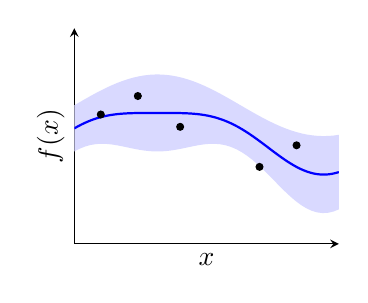
\begin{tikzpicture}[scale=0.62]
        \begin{axis}[
            xlabel={$x$},
            ylabel={$f(x)$},
            ticks=none,
            axis lines=left,
            ymin=-3, ymax=4,
            xmin=0, xmax=5,
            height=6cm, width=7cm,
        ]
          \addplot[name path=A, draw=none, domain=0:5, samples=50] {sin(deg(x)) + 1.5};
          \addplot[name path=B, draw=none, domain=0:5, samples=50] {sin(deg(x)) - 0.5 + 0.5*cos(deg(x)*2)};
          \addplot[fill=blue!15, draw=none, forget plot] fill between[of=A and B];
          \addplot[blue, thick, domain=0:5, samples=100, forget plot]
            {sin(deg(x)) + 0.5 + 0.25*cos(deg(x)*2)};
          \addplot[only marks, mark=*, mark size=2pt, color=black, forget plot] coordinates {
            (0.5, 1.2) (1.2, 1.8) (2.0, 0.8) (3.5, -0.5) (4.2, 0.2)
          };
        \end{axis}
      \end{tikzpicture}
    \end{column}
  \end{columns}
\end{frame}

% == A6 [TAX: Uncertainty] ==
\begin{frame}[fragile]{Appendix: Uncertainty (Shock Processes)}
\small
\begin{itemize}
    \item $\kappa_t$ follows an AR(1) process $\kappa_t = \rho_t \kappa_{t-1} + \epsilon_{\kappa,t}$ with $\kappa_0 = 0.3502$ and $\rho_t =  \rho_0 + (\rho_\infty - \rho_0) (1-\exp(- \delta^\rho  5t))$.
   \item $\epsilon_{\kappa,t}$ is discretized as:
    \begin{equation}
        \epsilon_{\kappa, t} =
\begin{cases}
0.03 & \text{with prob } 1/3, \\
0.0 & \text{with prob } 1/3, \\
- 0.03 & \text{with prob } 1/3.
\end{cases}
    \end{equation}
    \item $TP_t$ follows a random walk $TP_t = TP_{t-1} + \epsilon_{TP,t}$ with $TP_0 = 3.0$, $\epsilon_{TP,t}$ is discretized as:
    \begin{equation}
        \epsilon_{TP, t} =
\begin{cases}
0.1 & \text{with prob } 1/3, \\
0 & \text{with prob } 1/3, \\
- 0.1 & \text{with prob } 1/3.
\end{cases}
    \end{equation}
\end{itemize}
\end{frame}

% == A7 [TAX: Calibration] ==
\begin{frame}[fragile]{Appendix: Calibration}
\begin{table}[]
    \centering
    \small
    \begin{tabular}{ccc}
    \hline \hline
  \textbf{Symbol} & \textbf{Parameter} & \textbf{Value} \\
    \hline
    $\beta$  & Discount factor& 0.9 \\
    $\sigma$  & Relative risk aversion & 3 \\
    $\alpha$  & Capital share & 0.3 \\
    $\delta$  &Depreciation & 0.2 \\
    $\sigma_{ccr}$  & Climate sensitivity & 1.7 \\
    $\psi_1$  & parameter damage function & 13.16 \\
    $\theta_1$  & Intercept of control cost function & 0.7 \\
    $\theta_2$  & Exponent of control cost function & 2.6 \\
    $\kappa_{0}$  & Initial carbon intensity & 0.35032 \\
    $\rho_0$  & Initial AR(1) param for carbon intensity & 1.08 \\
    $\rho_{\infty}$  & Final AR(1) param for carbon intensity & 0.91 \\
    $\delta^{\rho}$  & AR(1) param depreciation for carbon intensity  & 0.04 \\
    $E_0$ & initial stock of carbon thGtC& 0.851 \\
    $L$ & Labor (to match initial emissions) & 600 \\
    \hline
\end{tabular}
    \caption{Parameterization of the OLG Model.}
    \label{tab:parameters}
\end{table}
\end{frame}

% == A8 [TAX: BAU Scenario versus RCP Scenarios] ==
\begin{frame}{Appendix: BAU Scenario versus RCP Scenarios}
    \centering
    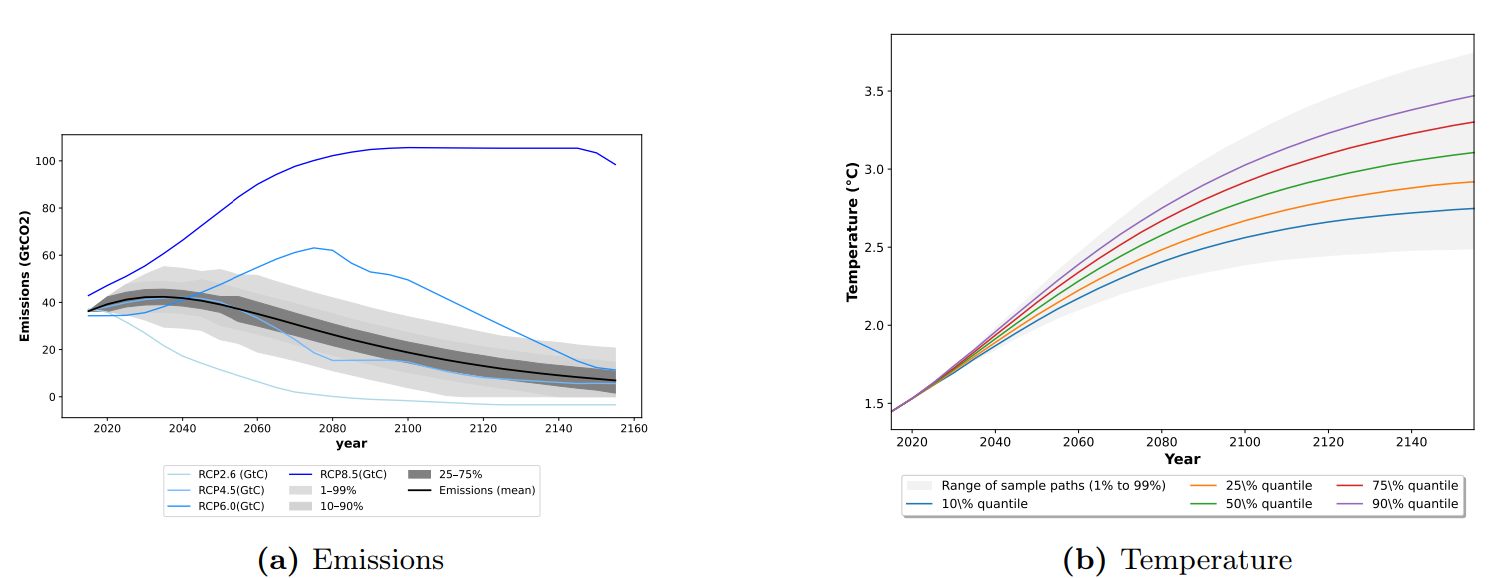
\includegraphics[width=0.7\textwidth, height=0.4\textheight, keepaspectratio]{tax/BAU_SOLG.png}

    \vspace{0.3em}
    \begin{columns}[t]
        \begin{column}{0.48\textwidth}
            \footnotesize
            \textbf{Left: Global CO$_2$ Emissions}
            \begin{itemize}
                \item Comparison of our model's BAU against IPCC Representative Concentration Pathways (RCP).
                \item Our endogenous emissions path tracks closely with \textbf{RCP 4.5}.
                \item Base year (0) corresponds to 2017.
            \end{itemize}
        \end{column}
        \begin{column}{0.48\textwidth}
            \footnotesize
            \textbf{Right: Global Warming Projections}
            \begin{itemize}
                \item Projected mean warming reaches $\approx \mathbf{3^\circ C}$ over 150 years.
                \item Substantial uncertainty exists: range of \textbf{2.5°C to 3.6°C}.
                \item Highlights significant tail risk in the absence of policy.
            \end{itemize}
        \end{column}
    \end{columns}
\end{frame}

% == A9 [TAX: Temperature (Scenario 1: Unconstrained)] ==
\begin{frame}{Appendix: Temperature (Scenario 1: Unconstrained)}
\begin{columns}[c]
    \begin{column}{0.5\textwidth}
        \centering
        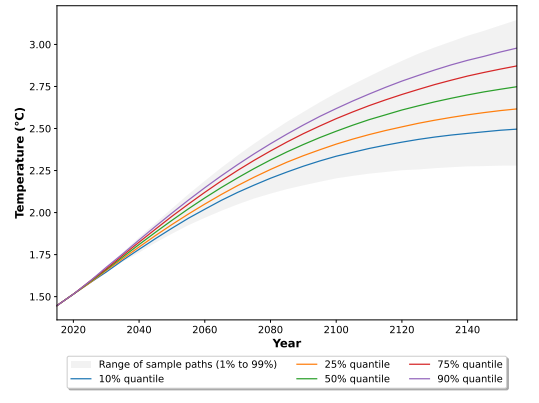
\includegraphics[width=0.92\linewidth]{tax/Temp_case1.png}
    \end{column}
    \begin{column}{0.47\textwidth}
        \small
        \textbf{Outcomes:}
        \begin{itemize}
            \setlength\itemsep{0.8em}
            \item \textbf{Aggressive Mitigation:} Stabilizes mean warming at \textbf{$\approx$2.7\,°C}.
            \item \textbf{Tail-Risk Insurance:} The 99th percentile is capped at $\approx$3.1\,°C.
            \item \textbf{The Mechanism:} Requires immediate, heavy taxation ($\approx$70\% average after 150 years).
            \item \textbf{The Cost:} Imposes up to \textbf{$-$5\% welfare losses} on current older cohorts.
        \end{itemize}
    \end{column}
\end{columns}
\end{frame}

% == A10 [TAX: Emissions (Welfare Maximizing)] ==
\begin{frame}{Appendix: Emissions (Welfare Maximizing)}
\begin{columns}[c]
    \begin{column}{0.55\textwidth}
        \centering
        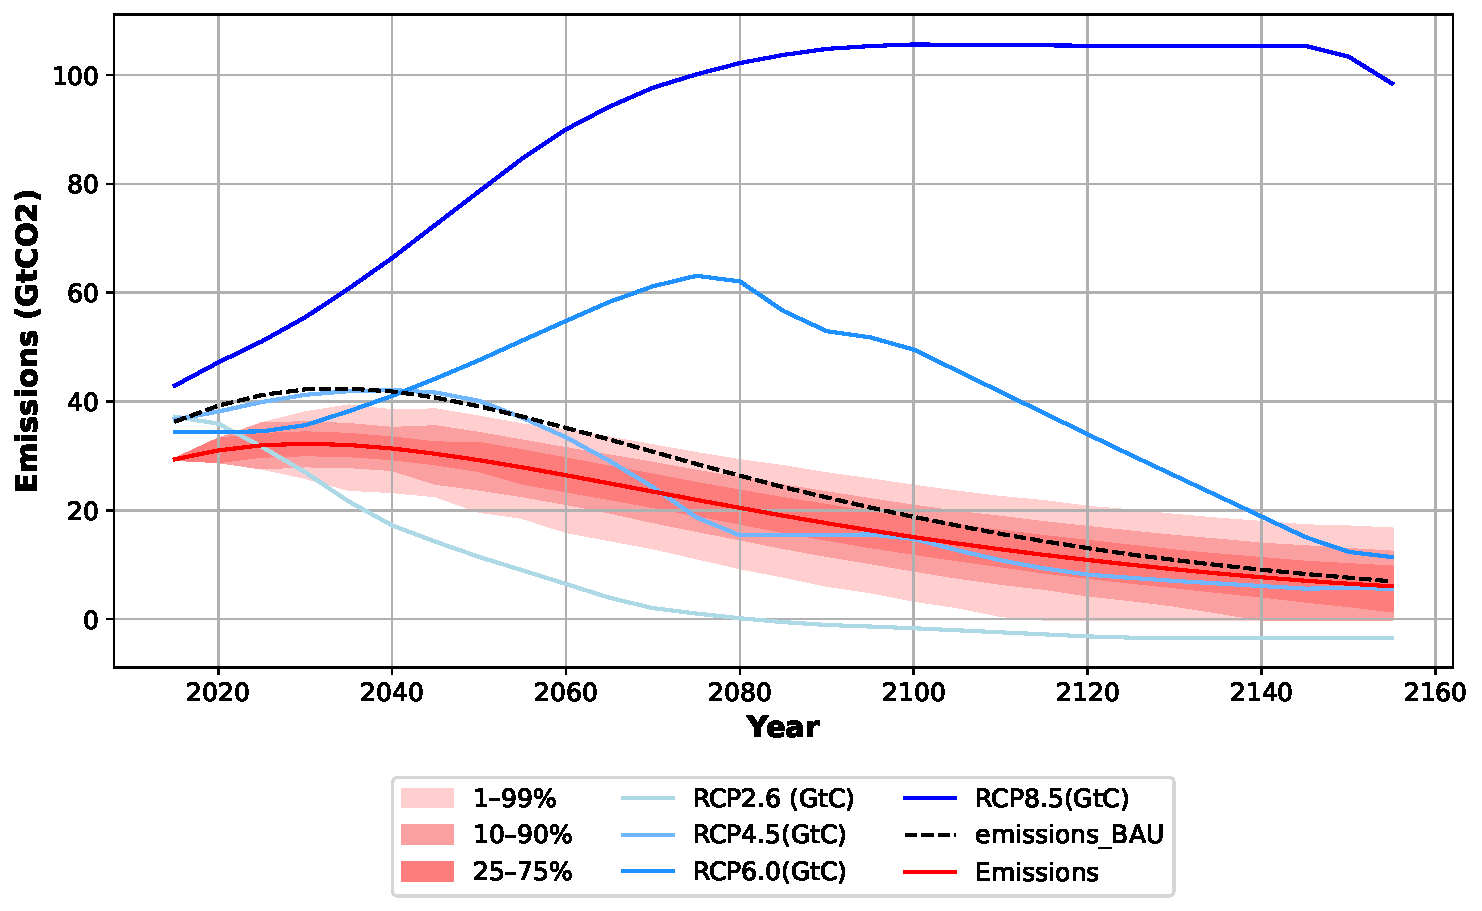
\includegraphics[width=0.92\linewidth]{tax/paper/lin_S_10trans_unif_emissions.pdf}
    \end{column}
    \begin{column}{0.42\textwidth}
        \small
        \begin{itemize}
            \setlength\itemsep{1em}
            \item \textbf{Immediate Shock:} Emissions drop $\approx \mathbf{25\%}$ below BAU within the first 50 years.
            \item \textbf{Eliminating the Extremes:} The policy successfully truncates the high-emission tail (the red shaded area).
            \item \textbf{Convergence:} Post-2100, the gap narrows as exogenous carbon intensity declines naturally.
        \end{itemize}
    \end{column}
\end{columns}
\end{frame}

% == A11 [TAX: Emissions: Mitigating Risk] ==
\begin{frame}{Appendix: Emissions: Mitigating Risk (Scenario 2)}
\begin{columns}
    \begin{column}{0.55\textwidth}
        \begin{figure}[th!]
            \centering
            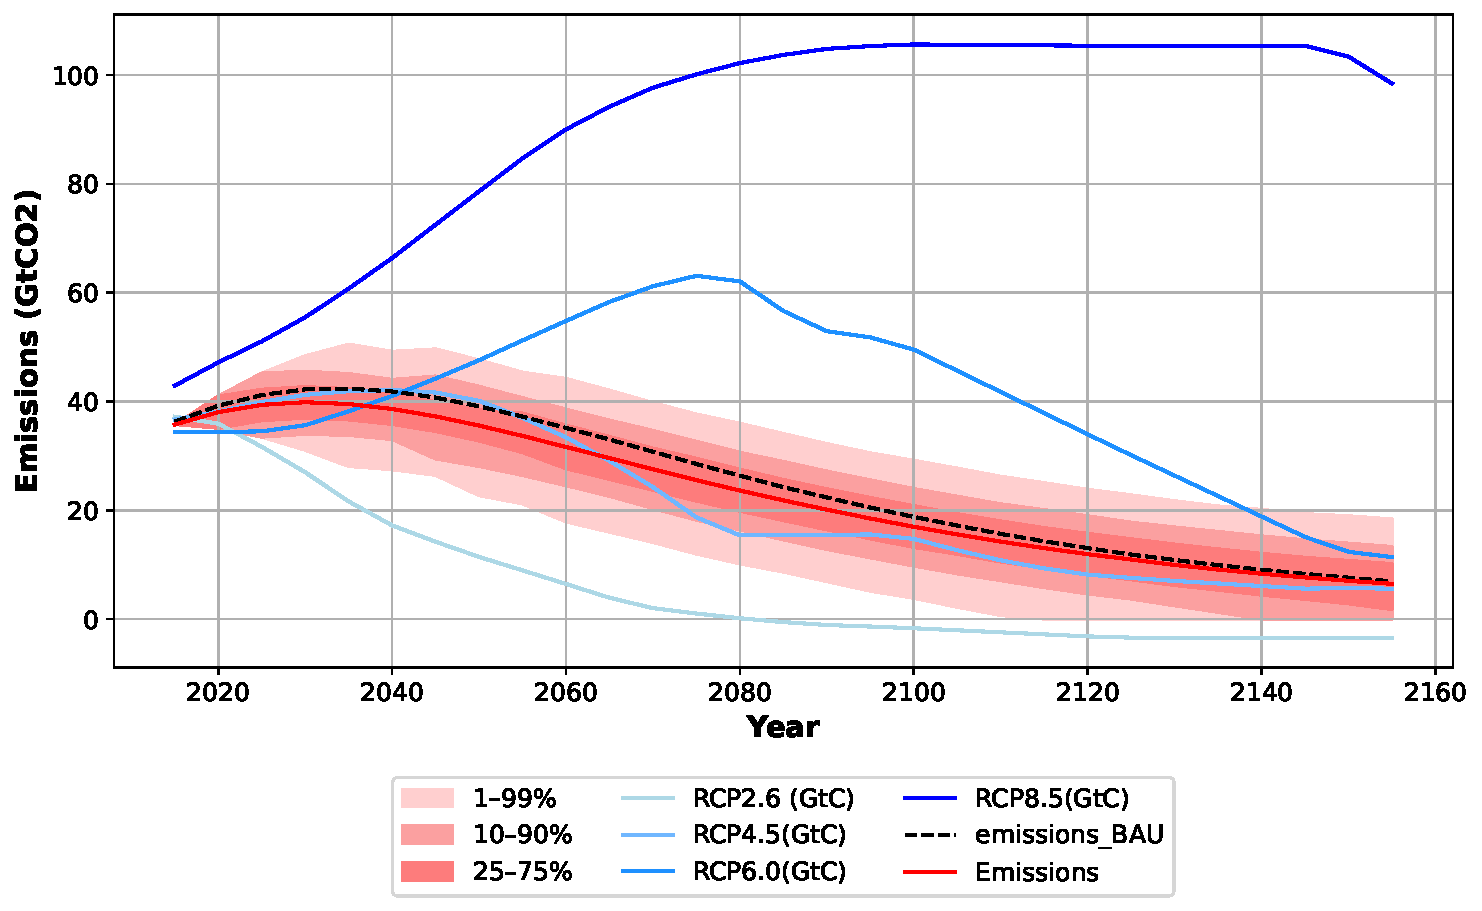
\includegraphics[width=0.92\linewidth]{tax/paper/lin_S_trans_emissions_dist.pdf}
        \end{figure}
    \end{column}
    \begin{column}{0.42\textwidth}
        \footnotesize
        \begin{itemize}
             \setlength\itemsep{0.9em}
            \item \textbf{Modest Average Reduction:} The mean emissions path is not drastically lower than BAU (required to preserve current consumption).
            \item \textbf{Tail Truncation:} The policy's primary physical impact is eliminating the high-emissions upside.
            \item \textbf{Result:} The $99^{th}$ percentile of emissions drops below $40~GtCO_2$ by 2070 (20 years earlier than BAU).
        \end{itemize}
    \end{column}
\end{columns}
\end{frame}

% == A12 [TAX: Appendix: Sampling Domain] ==
\begin{frame}[fragile]{Appendix: Sampling Domain}
\begin{table}[ht!]
\centering
\small
\begin{tabular}{lllll}
\toprule
Model & Planner Target & Parameter & $\underline{\vartheta_i}$ & $\bar{\vartheta_i}$ \\
\midrule
Linear in E & Max. Welfare & $\vartheta_0$     & -2.0   & 2.0   \\
            & Max. Welfare & $\vartheta_E$     & -2.0   & 2.0  \\
           & Max. Welfare & $\tau$         & 0.0  & 1.5  \\
            \midrule
Linear in E + Transfers & Pareto & $\vartheta_0$ & -0.5 & 0.1 \\
                        & Pareto & $\vartheta_E$ & 0.0    & 0.5 \\
                        & Pareto & $\tau$         & 0.0  & 0.8  \\
\midrule
Full linear + Transfers & Pareto & $\vartheta_0$     & -1.0   & 0.5 \\
                        & Pareto & $\vartheta_E$     & -0.5 & 1.0   \\
                        & Pareto & $\vartheta_\kappa$ & -0.6 & 0.6 \\
                        & Pareto & $\vartheta_{TP}$   & -1.0   & 1.0   \\
                        & Pareto & $\tau$         & 0.0  & 0.8  \\
\bottomrule
\end{tabular}
\caption{Parameter bounds across models and objectives.}
\label{tab:param_bounds_main}
\end{table}
\end{frame}

% == A13 [TAX: An Incomplete List of Related Literature (block version)] ==
\begin{frame}{Appendix: An Incomplete List of Related Literature}
    \footnotesize
    \begin{block}{Climate Risk in OLG Models}
        Existing work studies intergenerational conflict and climate damages \citep{kotlikoff2021making, weitzman2012ghg, Karp2014}.
        \begin{itemize}
            \item[\textcolor{blue}{\textbf{+}}] \textbf{Our Gap:} Most rely on linearization or ignore the \textit{political constraint} of Pareto improvements under uncertainty (e.g., tipping points).
        \end{itemize}
    \end{block}
    \begin{block}{Optimal Ramsey Policy with Heterogeneity}
        Established frameworks for fiscal/monetary policy in HA models \citep{bhandari2013taxes, nuno2020Optimal, douenne_hummel_pedroni_2024}.
        \begin{itemize}
             \item[\textcolor{blue}{\textbf{+}}] \textbf{Our Gap:} We enforce \textit{simple rules} (linear taxes) to make the policy implementable and interpretable.
        \end{itemize}
    \end{block}
    \begin{block}{Deep Learning for High-Dimensional Dynamic Stochastic Models}
        Using Neural Networks (DEQN) and Surrogates to beat the curse of dimensionality \citep{azinovic_et_al_2019, friedlDeep2023}.
        \begin{itemize}
             \item[\textcolor{blue}{\textbf{+}}] \textbf{Our Innovation:} A 3-step framework: DEQN (Global Solution) $\to$ GP Surrogate $\to$ Constrained Optimization.
        \end{itemize}
    \end{block}
\end{frame}

% =====================================================================
% Appendix section: the same surrogate quantifies uncertainty (UQ of the SCC)
% =====================================================================
% (appendix material -- not part of the timed main session)
\section{Appendix: UQ of the SCC}

% == F14: divider ==
{\setbeamercolor{background canvas}{bg=uzhgreylight}
\begin{frame}
\Huge \textcolor{uzhblue}{Appendix: How Uncertain Is the Social Cost of Carbon?}\\[0.5em]
{\normalsize \textcolor{uzhblue}{The \emph{quantify} operator on the same two-surrogate pipeline}}
\end{frame}}

% == F15 [UQ: Integrated Assessment Models (IAMs)] ==
\begin{frame}
\frametitle{Integrated Assessment Models (IAMs)}
\begin{itemize}
\item Pioneered by Nordhaus (DICE, RICE): Quantitative, often numerical.
\item Key components:
\begin{itemize}
    \item (Simplified) climate system.
    \item (Stylized) economic model of emissions AND damages.
\end{itemize}
\item Economic model: needs to be dynamic, forward-looking, possibly allowing stochasticity (temperature variations, disasters, TFP), and potentially heterogeneous agents (``who is how impacted?'').
\end{itemize}
\vfill
\begin{figure}[h]
\centering
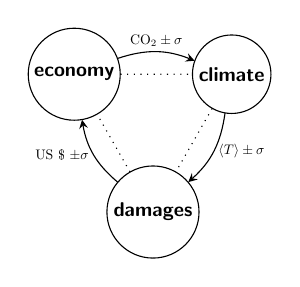
\begin{tikzpicture}[>=stealth, node distance=2cm, scale=0.5, transform shape]
    \tikzstyle{main node} = [circle, draw, minimum size=1cm, font=\sffamily\Large\bfseries]
    \node[main node] (economy) at (0,0) {economy};
    \node[main node] (climate) at (4,0) {climate};
    \node[main node] (damages) at (2,-3.5) {damages};
    \draw[->] (economy) to[bend left=20] node[above] {CO$_2 \pm \sigma$} (climate);
    \draw[->] (climate) to[bend left=20] node[right] {$\langle T \rangle \pm \sigma$} (damages);
    \draw[->] (damages) to[bend left=20] node[left] {US \$ $\pm \sigma$} (economy);
    \draw[dotted] (economy) -- (climate) -- (damages) -- (economy);
\end{tikzpicture}
\caption{Stylized representation of an IAM.}
\label{fig:IAM_stylized}
\end{figure}
\end{frame}

% == F16 [UQ: A Stochastic IAM with Bayesian Learning about the ECS] ==
\begin{frame}
\frametitle{A Stochastic IAM with Bayesian Learning about the ECS}
\resizebox{0.48\linewidth}{!}{
  \begin{minipage}{\linewidth}
\begin{align*}
  & V\left(\bm{X}_t\right)^{1-1/\psi}
  = \max_{C_{t},K_{t+1},\mu_{t}}\left\{\left( \frac{C_{t}}{L_{t}} \right)^{1-1/\psi}L_{t}
    +
    e^{-\rho} \mathbb{E}_{t}\left[V\left(\bm{X}_{t+1}\right)^{1-\gamma}\right]^{\frac{1-1/\psi}{1-\gamma}}\right\}
  \\
  \text{s.t.} \quad
  &
    \left(1-\Theta\left(\mu_{t}\right)\right)\Omega_t\left(T_{\mathrm{AT},t}\right)K_{t}^{\alpha}\left( A_{t}L_{t} \right)^{1-\alpha}
    - C_{t} - I_{t} = 0 \\
  &  \left( 1-\delta \right)K_{t} + I_{t} - K_{t+1} = 0\\
  &  1 - \mu_{t} \geq 0  \\
  &
  \left(1-\phi_{12}\right)M_{\mathrm{AT},t}+\phi_{21}M_{\mathrm{UO},t}+\left(1-\mu_{t}\right)\sigma_{t}K_{t}^{\alpha}\left( A_{t}L_{t} \right)^{1-\alpha} + E_{\mathrm{Land},t} - M_{\mathrm{AT},t+1} = 0 \\
      &
    \phi_{12}M_{\mathrm{AT},t}+\left(1-\phi_{21}-\phi_{23}\right)M_{\mathrm{UO},t}+\phi_{32}M_{\mathrm{LO},t}
  - M_{\mathrm{UO},t+1} = 0 \\
  &
    \phi_{23}M_{\mathrm{UO},t}+\left(1-\phi_{32}\right)M_{\mathrm{LO},t} -
    M_{\mathrm{LO},t+1} = 0 \\
& \nonumber
\left( 1 - \varphi_{21} - \varphi_{1C}\right)T_{\mathrm{AT},t}+\varphi_{21}T_{\mathrm{OC},t}
+ \varphi_1 \left(F_{\mathrm{2xco2}} \log_2 \left(\frac{M_{\mathrm{AT},t}}{M_{\mathrm{AT}}^\ast} \right)+F_{\mathrm{EX},t} \right) +  \\
&
\qquad \varphi_{1C}\tilde{f}_{t+1}T_{\mathrm{AT}, t} + \tilde{\epsilon}_{T, t+1} - T_{\mathrm{AT},t+1} = 0
 \\
&
\varphi_{4}T_{\mathrm{AT},t}+\left(1-\varphi_{4}\right)T_{\mathrm{OC},t}
  -  T_{\mathrm{OC},t+1} = 0 \\
 &
  \frac{
 S_{\epsilon_{T}} \mu_{f,t} +  \varphi_{1C} T_{\mathrm{AT}, t}  \left( \varphi_{1C} T_{\mathrm{AT}, t} \tilde{f}_{t+1} + \tilde{\epsilon}_{T,t+1}  \right) S_{f, t}}{S_{\epsilon_{T}} + \left(\varphi_{1C} T_{\mathrm{AT}, t} \right)^2 S_{f, t} } - \mu_{f,t+1} = 0\\
&
 \frac{S_{\epsilon^{T}} S_{f, t}}{S_{\epsilon^{T}} + \left( \varphi_{1C} T_{\mathrm{AT}, t} \right)^{2} S_{f, t}}  - S_{f, t+1} = 0 \\
&
\tilde{f}_{t+1} \sim \mathcal{N}\left( \mu_{f,t}, S_{f, t}, \underline{f}, \overline{f} \right),
\tilde{\epsilon}_{T,t+1} \sim \mathcal{N}\left( 0, S_{\epsilon^T} \right)
\end{align*}
\end{minipage}
}

\begin{footnotesize}
\begin{itemize}
    \item $X_{t} = \left[ k_{t}, M_{\mathrm{AT}, t}, M_{\mathrm{UO}, t}, M_{\mathrm{LO}, t}, T_{\mathrm{AT}, t}, T_{\mathrm{OC}}, \mu_{f,t}, S_{f,t}, t; \theta\right]$.
    \item \keyc{Minimal model has a \textbf{9+N}-dimensional state space}.
    \item Uncertain equilibrium climate sensitivity following \cite{roe2007climate}: climate feedback $f \sim \mathcal{N}(\mu_f, S_f)$; details in the appendix.
\end{itemize}
\end{footnotesize}
\end{frame}

% == F17 [UQ: Parameter Ranges for the UQ Analysis], verbatim ==
\begin{frame}[fragile]{Parameter Ranges for the UQ Analysis}
\begin{table}
\label{table:param_UQ}
\centering
\begin{tabularx}{\linewidth}{lllll}
\toprule
Parameter &  $\theta^{0}_{i}$ &
$\underline{\theta}_{i}$&  $\overline{\theta}_{i}$ & Source
  etc.\\
\midrule
$\rho$ & 0.015 & 0.01 & 0.02 & {\citet{stern2007economics}}\\
$\gamma$ & 10. & 5.0 & 10.0 & \makecell[l]{\citet{jensen_traeger_2014} and \\ \citet{Cai_Lontzek_2019}}\\
$\psi$ & 1.5 & 0.5 & 2.0 & --//-- \\
$\pi_{2}$ & 0.00236 & 0.002  & 0.008 & \makecell[l]{\citet{nordhaus2017revisiting} and \\ \citet{weitzman2012ghg}}\\
$\mu_{f,0}$  & 0.65 &  0.45 & 0.73 & \citet{roe2007climate}\\
$S_{f,0}$  & 0.0169 & 0.01 & 0.04 & \citet{roe2007climate}\\
\bottomrule
\end{tabularx}
\end{table}
\vspace{0.3em}
{\footnotesize These are the uncertain $\bm{\theta}$ entering the surrogate as pseudo-states.}
\end{frame}

% == F18 [UQ: B-MAP: Deep Equilibrium Nets & IAMs + Why Surrogate Models?], trimmed ==
\begin{frame}{Instantiating the Pipeline: Parameters as Pseudo-States}
\small
\begin{itemize}\itemsep4pt
\item  \keyc{DEQNs can solve nonlinear stochastic models globally, even if geometry is oddly-shaped, in minutes to hours on a laptop}; state spaces up to dozens of variables.
\item Add pseudo-states for uncertainty quantification at a small extra cost: \keyc{only one \textbf{single} model evaluation needed}: here the pseudo-states are the structural parameters $\bm{\theta}$, the move Session 2 made with $\varrho$ and $\beta$.
\item The computed policies are functions of this extended state space; to obtain QoIs as a function of the parameters, simulate the economy with the derived policy functions to compute the SCC at $N$ points.
\item The remaining UQ tasks are just ``post-processing'', and come at low computational costs, as we can query a \key{surrogate} (Surrogate 2, fitted to those $N$ points).
\end{itemize}
\end{frame}

% == F19 [UQ: Social Cost of Carbon - Learning Matters] ==
\begin{frame}[fragile]{The QoI: Social Cost of Carbon [\$/tonC]}
{\small The SCC: the marginal loss caused by an extra ton of CO$_2$ emissions; the level of the carbon tax is based on it. Computed here from surrogate simulations.}
\begin{figure}
    \centering
        
\includegraphics[width=0.44\textwidth]{uq/nolearn_trunc/benchmark/distribution_2015-2100_scc.pdf}
    
\includegraphics[width=0.44\textwidth]{uq/learn_trunc/benchmark/distribution_2015-2100_scc.pdf}
\end{figure}
{\small Model with no learning (left) and learning (right); SCC behaves like a random variable, as Temperature and ECS are stochastic (our results confirm~\cite{Cai_Lontzek_2019}).}
\end{frame}

% == F20 [UQ: Why Global UQ? + Global UQ: 3 Quantities], merged ==
\begin{frame}{Global Sensitivity Analysis: 3 Quantities}
\small
\begin{itemize}\itemsep3pt
    \item \textbf{\emphc{How are quantitative results of IAMs sensitive to a specific parameterization}}? A \key{importance ranking} informs the researcher on which parts to focus when calibrating or extending a model, or the policymaker on which parameters need further scrutiny.
    \item ``One-at-a-time'' approaches tend to be unstructured and are only \textbf{local}: highly dependent on the chosen parameter values. We aim at determining which input parameters (or combinations) contribute the most to the uncertainty of the QoI, globally.
	\item Measures we use:
	\begin{itemize}
	    \item \keyc{\textbf{Sobol' index}: prioritization of the uncertain parameters based on the outcome variance explained}.
        \item \keyc{\textbf{Shapley value}: identifies how much model variance can be attributed to the uncertainty in input parameters}.
        \item \keyc{\textbf{Univariate effect}: shows how each parameter affects the outcomes}.
	\end{itemize}
\end{itemize}
$\rightarrow$ All three are computed on a cheap-to-evaluate \textbf{surrogate model} based on Gaussian Processes~\citep{scheideggerbilinois_2019}, e.g., SCC($\theta_1, \theta_2,...,\theta_N$).
\end{frame}

% == F21 [UQ: Univariate Effect (UE)] ==
\begin{frame}{Univariate Effect (UE)}
\small
\begin{itemize}\itemsep4pt
 \item UE: measures the non-linear relationship between the target QoI and an uncertain input parameter.
    \item UE is the conditional expectation, integrating over the other uncertain parameters $\theta_{-i}$, of the QoI as a function of an input parameter $\theta_{i}$ fixed at an arbitrary value $t$:\footnote{In the source figures the fixed value is denoted $\vartheta_i$; we reserve $\vartheta$ for policy parameters throughout this lecture.}
\begin{align*}
  \mathcal{M}^{ 1 }_{i}\left( t \right) =
  \mathbb{E}_{\theta_{-i}}\left[ Y \mid \theta_{i}=t  \right].
\end{align*}
\end{itemize}
\vspace{0.3em}
$\rightarrow$ Sobol' indices do not include information about the direction in which a parameter affects the quantities of interest.

$\rightarrow$ Univariate effects help to find regions of high and low sensitivity, and can be interpreted as a robust direction of change under parameter uncertainty.
\end{frame}

% == F22 [UQ: Learning: Univariate effects on the SCC in 2020] ==
\begin{frame}
\frametitle{Univariate Effects on the SCC in 2020 (Learning Model)}
\begin{figure}
    \centering
    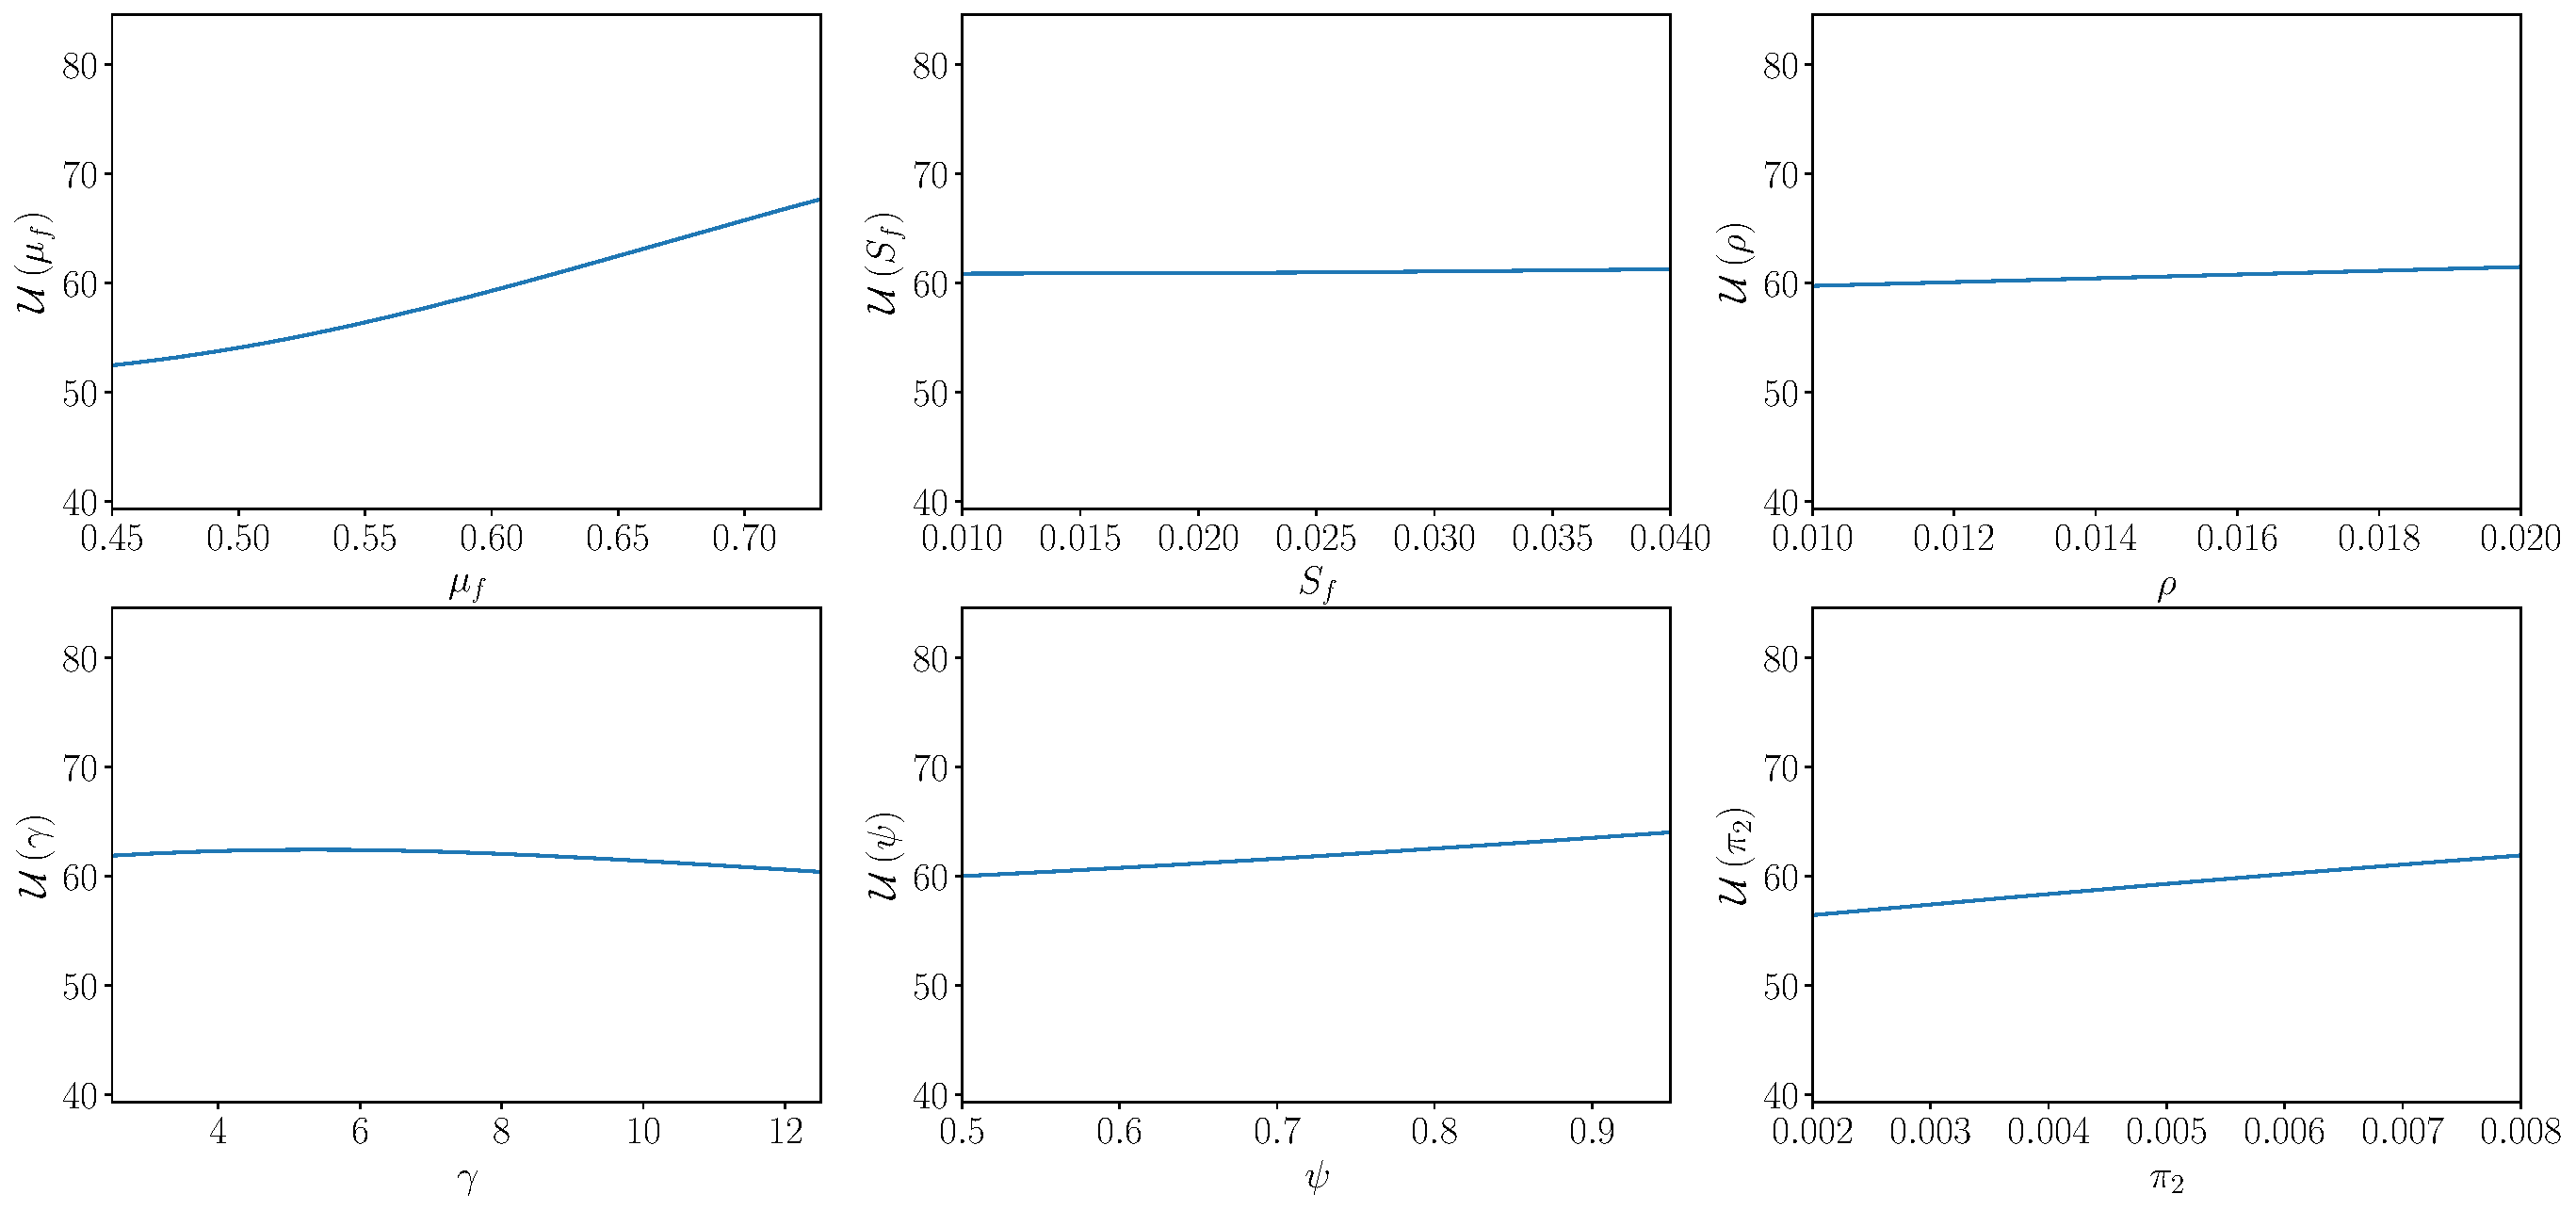
\includegraphics[width=0.92\textwidth]{uq/Learning_upd/uni_pred_E_scc2020_panel.pdf}
\end{figure}
\end{frame}

% == F23 [UQ: Sobol' indices + When to use Sobol' indices?], merged ==
\begin{frame}{Sobol' Indices}
\small
\begin{itemize}\itemsep3pt
    \item Consider a generic model $\mathcal{M}\left( \cdot \right)$ with $N$ uncertain input parameters $\theta$ and output $y$ summarizing the QoI (e.g., SCC):
    \begin{align*}
      \theta \in \mathcal{D}_{\theta} \subset \mathbb{R}^{N} \mapsto y =
      \mathcal{M}\left( \theta_{1}, \theta_{2},\cdots,\theta_{N} \right)
      \in \mathbb{R}^{Q}.
    \end{align*}
    \item The first-order Sobol' indices are defined as:\footnote{For simplicity, we assume $Q=1$.}
    \begin{align*}
    S_{i} \equiv \frac{\mathrm{Var}_{\theta_{i}}\left[ \mathbb{E}_{\Theta \setminus \theta_{i}}\left[ y \mid \theta_{i} \right] \right]}{\mathrm{Var}_{\Theta}\left[ y \right]}
    \end{align*}
    \item The numerator measures the first-order effect of $\theta_{i}$ on the model output $y$; normalizing by the total model variance $\mathrm{Var}_{\Theta}\left[ y \right]$ scales the index to $[0, 1]$.
    \item \textbf{Screening interpretation:} the first-order Sobol' index indicates by what percentage the total variance would be reduced, should the parameter $\theta_i$ be perfectly known and set to a fixed value. If it is small (in practice $< 1\%$), $\theta_i$ can be set to a deterministic value without changing the distribution of the QoI.
\end{itemize}
\end{frame}

% == F24 [UQ: Importance of Parameters for SCC in 2020] ==
\begin{frame}
\frametitle{Importance of Parameters for SCC in 2020}
\begin{figure}
    \centering
        
\includegraphics[width=0.46\textwidth]{uq/nolearn_uq/shapley_S1st_GP_E_scc2020.pdf}
    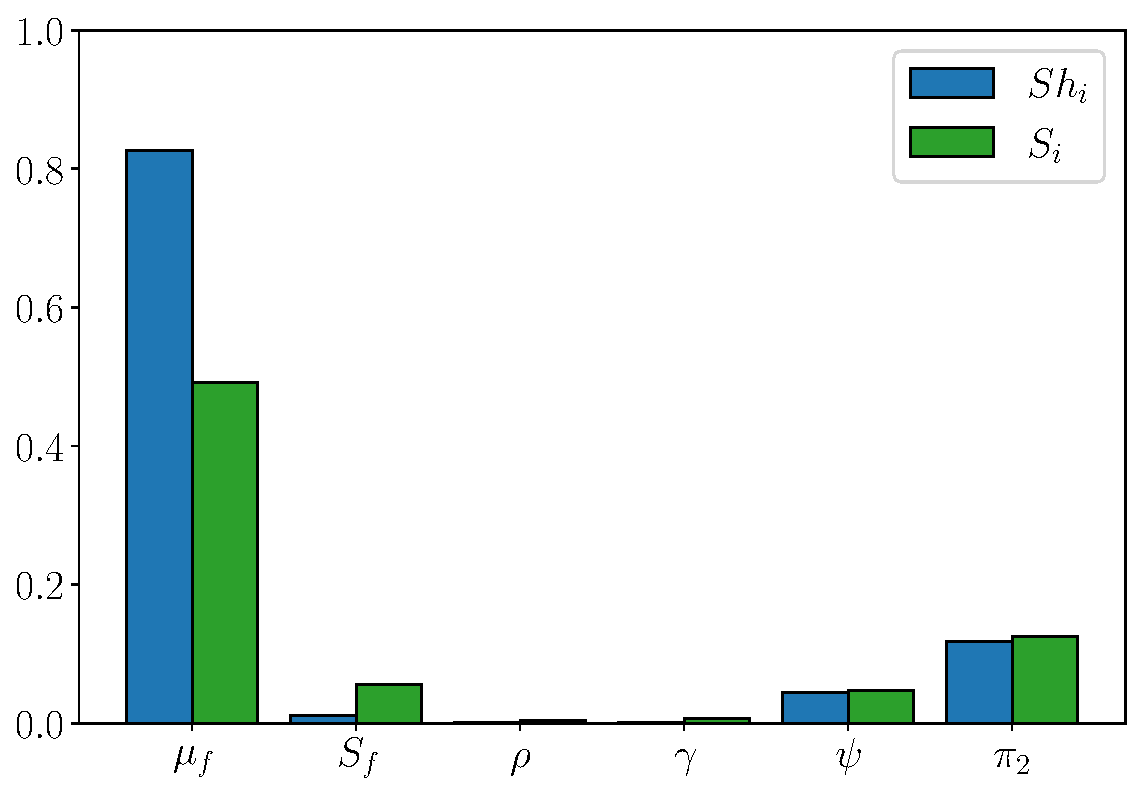
\includegraphics[width=0.46\textwidth]{uq/Learning_upd/shapley_S1st_GP_E_scc2020.pdf}
\end{figure}
UQ results (Shapley values and first-order Sobol' indices) for the model without learning (left) and with learning (right) in 2020.
\end{frame}

% == F25 [UQ: Conclusion & Outlook], takeaways verbatim ==
\begin{frame}{UQ Takeaways: What Drives SCC Uncertainty}
\begin{itemize}\itemsep6pt
	\item Uncertainty in SCC is mainly driven by parametric uncertainty in the ECS and the damage function.
 	\item Overall, highly nuanced results.
    \item The quantify operator ran entirely in post-processing: the equilibrium was solved exactly once.
    \item \textbf{Some open-source codes here}:
    \begin{itemize}
        \item \url{https://github.com/ClimateChangeEcon/Climate_in_Climate_Economics}
        \item \url{https://github.com/sischei/DeepEquilibriumNets}
    \end{itemize}
\end{itemize}
\end{frame}


% == A14 [UQ: The blue marble in 5 state variables] ==
\begin{frame}[fragile]{Appendix: The blue marble in 5 state variables
\begin{tikzpicture}[overlay, remember picture]
  \node[xshift=-1.6cm,yshift=-2.cm] at (current page.north east) {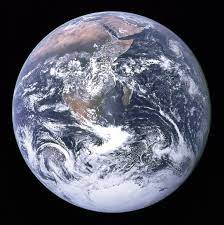
\includegraphics[width=1.6cm,height=1.6cm]{uq/earth.png}};
\end{tikzpicture}}
\begin{footnotesize}
\begin{minipage}{0.84\textwidth}
\begin{itemize}
\item Climate module: DICE-2016 functional form~\citep{Nordhaus2017}, calibrated to CMIP5 output~\citep{Folini_2021}.
\item \textbf{5 state variables} $=$ 3 carbon reservoirs $+$ 2 temperature layers.
\end{itemize}
\end{minipage}
\end{footnotesize}
\vspace{0.3cm}
\begin{columns}[t]
\begin{column}{0.44\textwidth}
{\footnotesize \textbf{Carbon cycle}: 3 reservoirs: Atmosphere (A), Upper ocean (U), Lower ocean (L).}

\vspace{0.2cm}
{\scriptsize
\begin{align*}
M_t &=(M_{A,t},M_{U,t},M_{L,t})^{\top}\\
M_{t+1} &= (I + \Delta_t B)\, M_{t} + \Delta_t E_{t}\\
E_t &= E_{\mathrm{ind},t} + E_{\mathrm{Land}}
\end{align*}}
\end{column}
\begin{column}{0.56\textwidth}
{\footnotesize \textbf{Energy balance}: 2 layers: atmosphere $T^{\mathrm{AT}}$, ocean $T^{\mathrm{OC}}$.}

\vspace{0.2cm}
\resizebox{\linewidth}{!}{$\displaystyle
\begin{aligned}
T^{\mathrm{AT}}_{t+1} &= T^{\mathrm{AT}}_{t} + \Delta_t c_{1}\!\left(F_{t} - \lambda T^{\mathrm{AT}}_{t} - c_{3}(T^{\mathrm{AT}}_{t} - T^{\mathrm{OC}}_{t})\right)\\
T^{\mathrm{OC}}_{t+1} &= T^{\mathrm{OC}}_{t} + \Delta_t c_{4}(T^{\mathrm{AT}}_{t} - T^{\mathrm{OC}}_{t})\\
F_{t} &= F_{\mathrm{2XCO2}}\, \tfrac{\log(M^{\mathrm{AT}}_{t}/M^{\mathrm{AT}}_{\mathrm{EQ}})}{\log 2} + F^{\mathrm{EX}}_{t}
\end{aligned}$}
\end{column}
\end{columns}
\vspace{0.3cm}
{\footnotesize $\rightarrow$ Emissions $E_t$ (economic activity $+$ exogenous land source) raise atmospheric carbon $M_{\mathrm{AT}}$, which drives the forcing $F_t$ and hence temperature $T^{\mathrm{AT}}$.}
\end{frame}

% == A15 [UQ: A Source of Uncertainty: Equilibrium Climate Sensitivity] ==
\begin{frame}
\frametitle{Appendix: A Source of Uncertainty: Equilibrium Climate Sensitivity}
\begin{figure}
 \centering
  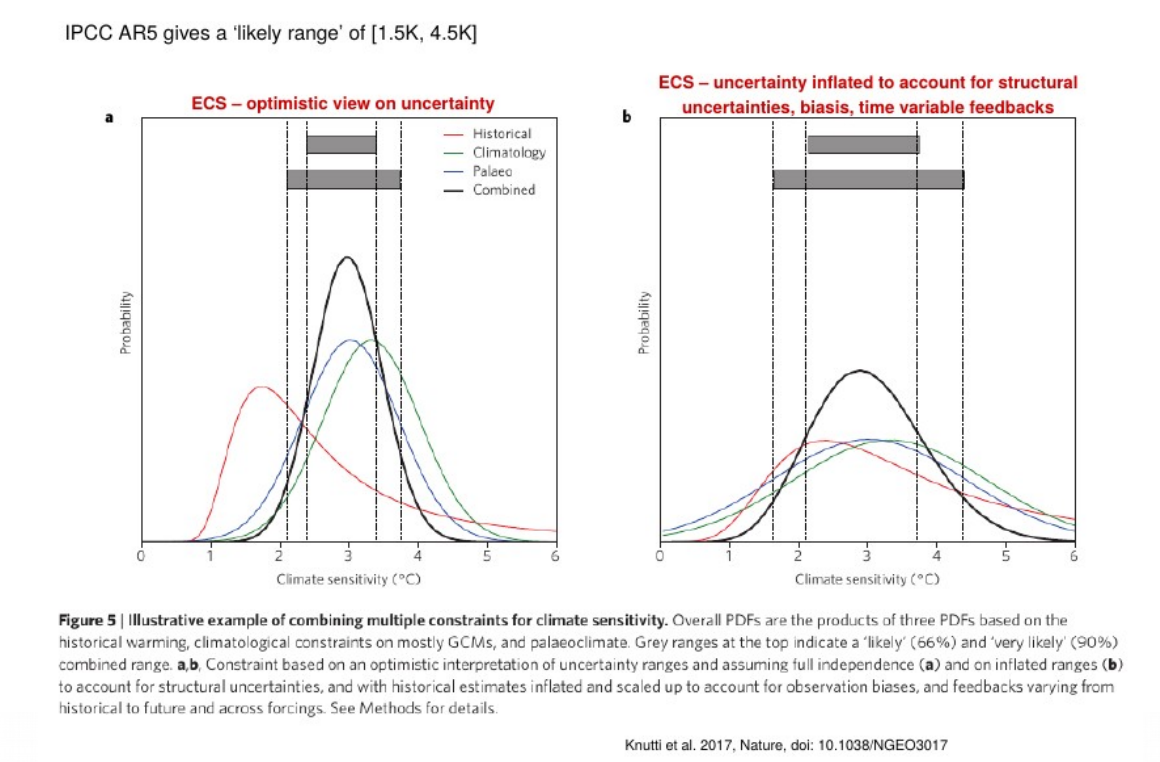
\includegraphics[height=0.7\textheight]{uq/knutti.png}
\end{figure}
\end{frame}

% == A16 [UQ: Another Source of Uncertainty: Damage Functions] ==
\begin{frame}
\frametitle{Appendix: Another Source of Uncertainty: Damage Functions}
\begin{figure}
 \centering
  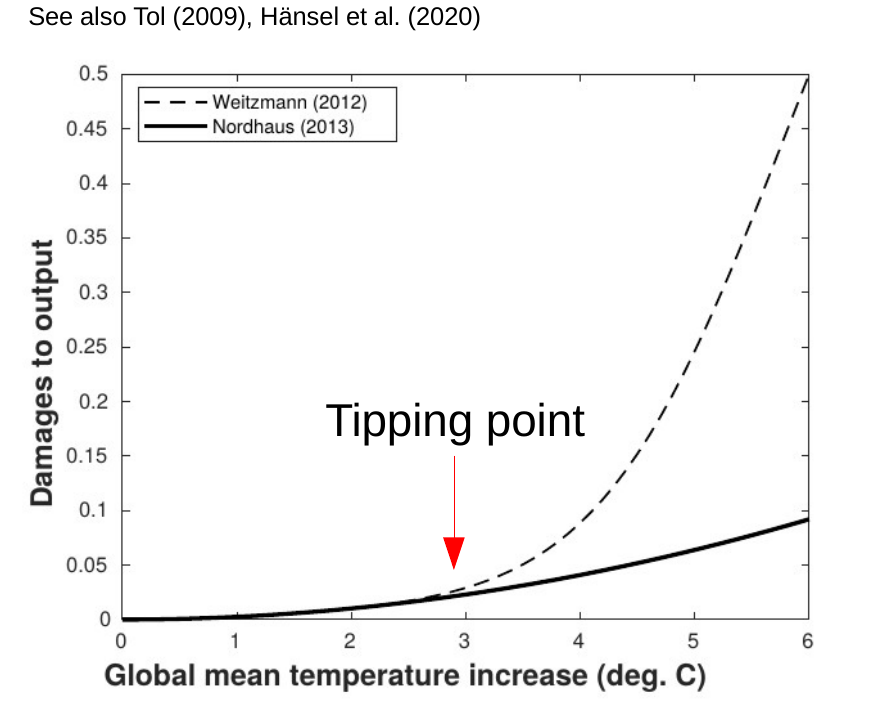
\includegraphics[width=0.18\textwidth]{uq/damge.png}
\end{figure}
\vspace{-0.5em}
    \begin{footnotesize}
\begin{itemize}
    \item Weitzman (2012):
    \begin{equation*}
 \Omega_t \left( T_{\mathrm{AT}, t} \right) =  \frac{1}{1 + \left(\frac{1}{\psi_1} T_{\mathrm{AT}, t} \right)^{2} + \left( \frac{1}{2 \cdot TP_{t}} T_{\mathrm{AT}, t} \right)^{6.754}}.
    \end{equation*}
    \item Nordhaus (2013):
    \begin{equation*}
\Omega^N_t \left( T_{\mathrm{AT}, t} \right) = \frac{1}{1 + {\pi_1} T_{\mathrm{AT}, t} +  {\pi_2} T_{\mathrm{AT}, t}^{2} }.
    \end{equation*}
    \item Degree of convexity is of key importance in determining the optimal taxes, not only the level.
    \item Tipping points: include losing much of the Amazon rain forest, faster onset of El Nino, the reversal of the Gulf Stream, etc.
\end{itemize}
    \end{footnotesize}
\end{frame}

% == A17 [UQ: Quantifying uncertainty about ECS] ==
\begin{frame}
\frametitle{Appendix: Quantifying uncertainty about ECS}
\small
\begin{itemize}
\item Temperature equation:
\begin{align}
T_{\mathrm{AT},t+1} = \left(1-\varphi_{21} - \varphi_1\frac{F_{\mathrm{2xco2}}}{\stoch{\Delta T_{\mathrm{AT},\times 2}}}\right)T_{\mathrm{AT},t}+\varphi_{21}T_{\mathrm{OC},t}+\\
\varphi_1 \left(F_{\mathrm{2xco2}} \log_2 \left(\frac{M_{\mathrm{AT},t}}{M_{\mathrm{AT}}^\ast} \right)+F_{\mathrm{EX},t} \right)
\end{align}
    \item Follow \cite{roe2007climate} to make ECS stochastic.
    \item $\mathrm{ECS}=\frac{\lambda_0}{1-f} F_{\mathrm{2XCO2}}$, with climate feedback parameter $ f \sim  \mathcal{N}\left(\mu_{f}, S_f \right) $.
\item  This is controversial, see \cite{zaliapin2010another} and \cite{roe2011comment} and \cite{zaliapin2011reply}.
\end{itemize}
\end{frame}

% == A18 [UQ: Bayesian learning mechanics] ==
\begin{frame}
\frametitle{Appendix: Bayesian learning mechanics}
\small
\begin{itemize}
    \item Temperature evolves as:
\resizebox{0.75\linewidth}{!}{
  \begin{minipage}{\linewidth}
      \begin{align*}
&T_{\mathrm{AT},t+1} = \left(\varphi_1\frac{F_{\mathrm{2xco2}}}{\Delta T_{\mathrm{AT},\times 2}^{0}} \stoch{\tilde{f}_{t+1}} + 1-\varphi_{21} - \varphi_{1}\frac{F_{\mathrm{2xco2}}}{\Delta T_{\mathrm{AT},\times 2}^{0}} \right)T_{\mathrm{AT},t}\\
&+\varphi_{21}T_{\mathrm{OC},t}+\varphi_1 \left(F_{\mathrm{2xco2}} \log_2 \left(\frac{M_{\mathrm{AT},t}}{M_{\mathrm{AT}}^\ast} \right)+F_{\mathrm{EX},t} \right) + \stoch{\tilde{\epsilon}_{T, t+1}}
\end{align*}
\end{minipage}}

where $\stoch{\tilde{f}_{t+1}} \sim \mathcal{N}\left( \mu_{f,t}, S_{f, t}, \underline{f}, \overline{f} \right)$: uncertain climate sensitivity,  $\stoch{\tilde \epsilon_{T, t+1}}$: shock to the temperature.
    \item The agent observes a realisation of the shocks in climate sensitivity and temperature at the beginning of the period $t$ before the decisions are made.
    \item Under Gaussian assumption analytic formulas for updating:
\resizebox{0.75\linewidth}{!}{
  \begin{minipage}{\linewidth}
    \begin{align*}
& \mu_{f,t+1} = \frac{
 S_{\epsilon_{T}} \mu_{f,t} +  \varphi_{1C} T_{\mathrm{AT}, t}  \left( \varphi_{1C} T_{\mathrm{AT}, t} \tilde{f}_{t+1} + \tilde{\epsilon}_{T,t+1}  \right) S_{f, t}}{S_{\epsilon_{T}} + \left(\varphi_{1C} T_{\mathrm{AT}, t} \right)^2 S_{f, t} }\\
 & S_{f, t+1} = \frac{S_{\epsilon_{T}} S_{f, t}}{S_{\epsilon_{T}} + \left( \varphi_{1C} T_{\mathrm{AT}, t} \right)^{2} S_{f, t}}
\end{align*}
\end{minipage}}
\end{itemize}
\end{frame}

% == A19 [UQ: Tail learning] ==
\begin{frame}[fragile]{Appendix: Tail learning}
\begin{figure}[t!]
\centering
\begin{subfigure}[t]{0.4\linewidth}
    \centering
    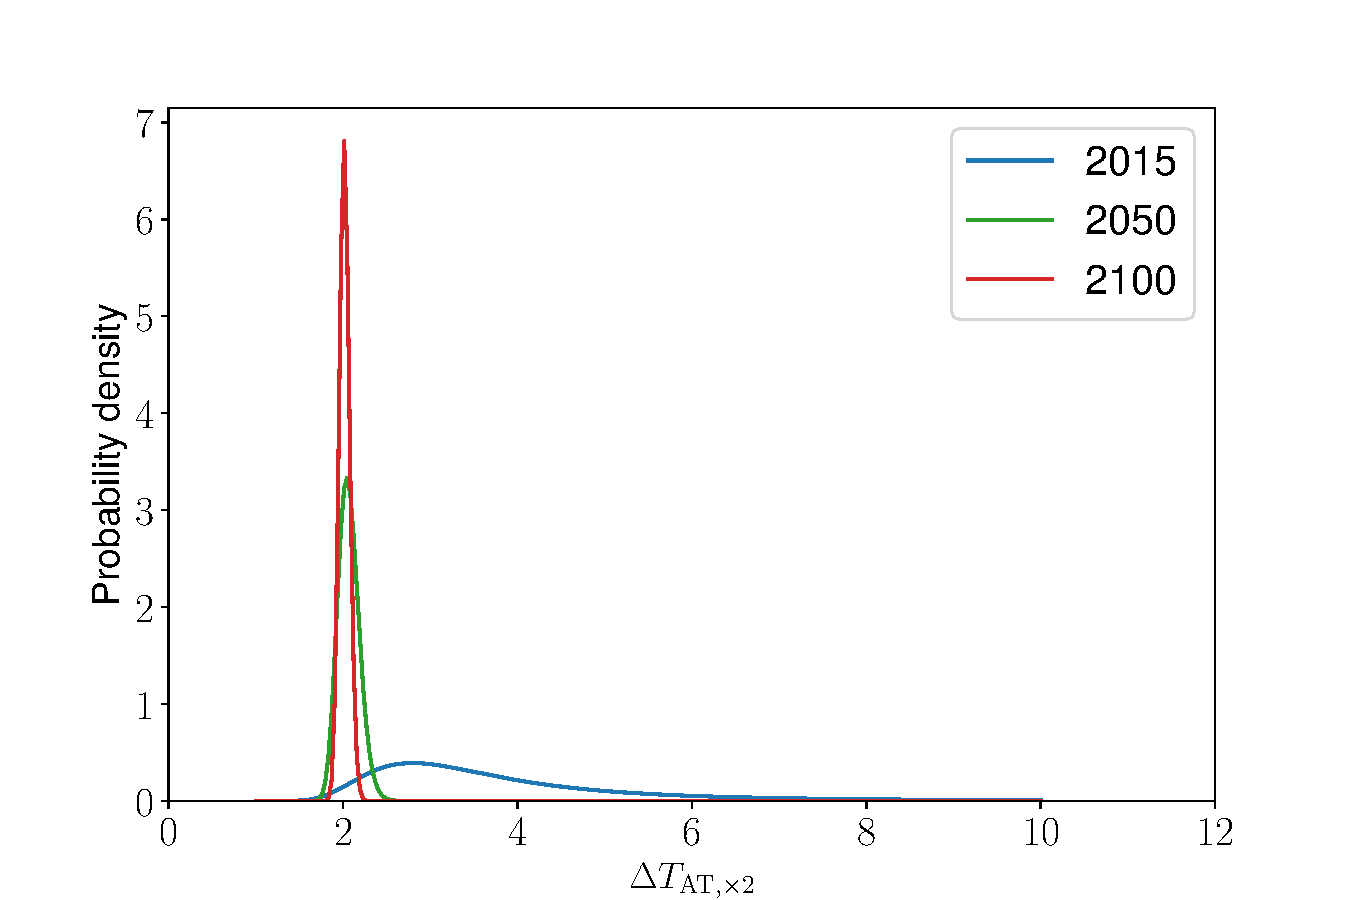
\includegraphics[width=1.0\linewidth]{uq/tail_learning/posterior_ECS_years_truef0.4.pdf}
    \caption{$\Delta T^{\ast}_{\mathrm{AT}, \times 2}=2.0$}
    \label{fig:posterior_distribution_ECS2.0}
\end{subfigure}
\hfill
\begin{subfigure}[t]{0.4\linewidth}
    \centering
    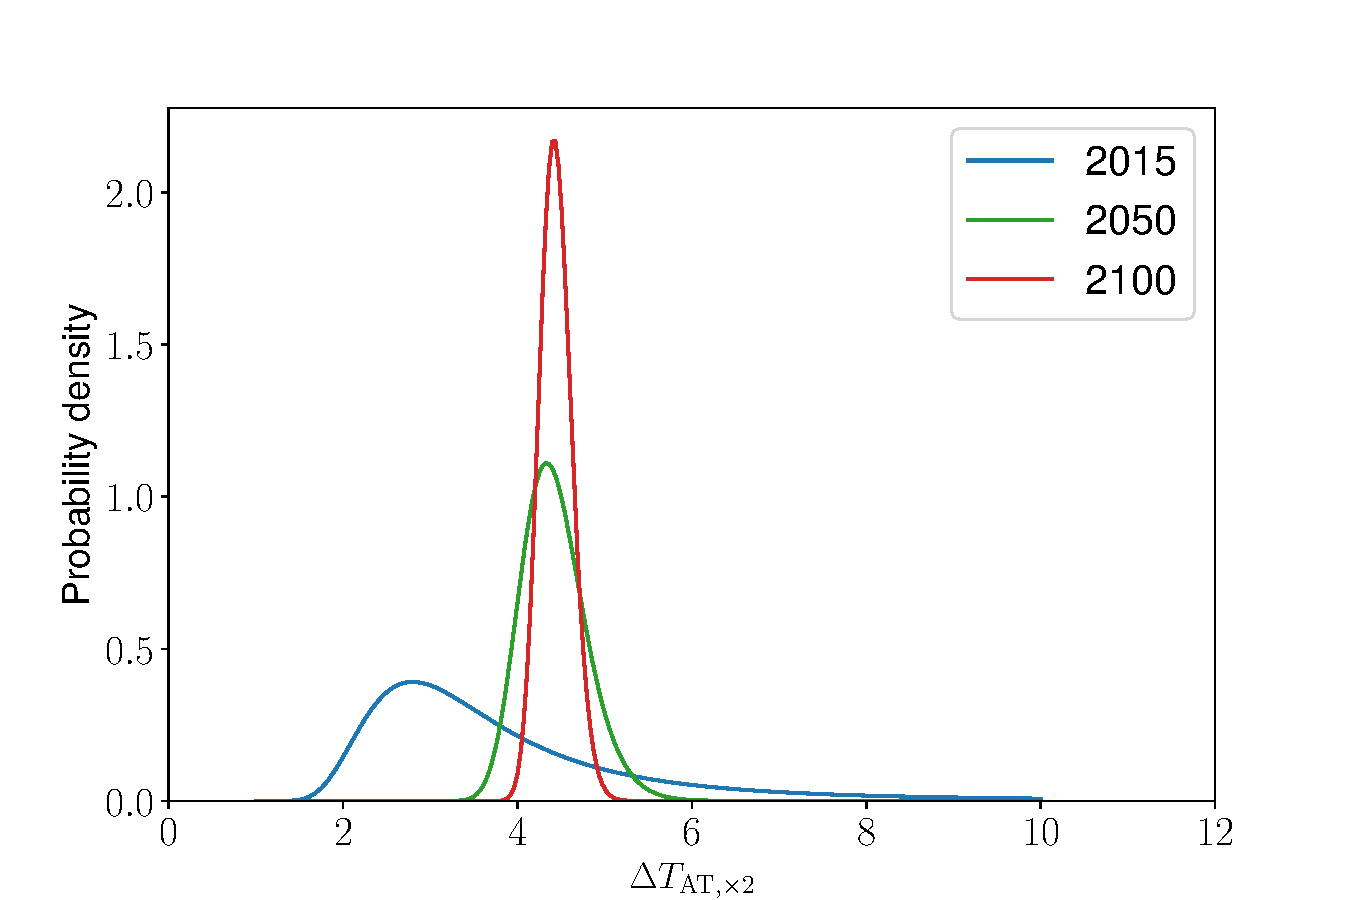
\includegraphics[width=1.0\linewidth]{uq/tail_learning/posterior_ECS_years_truef0.73.pdf}
    \caption{$\Delta T^{\ast}_{\mathrm{AT}, \times 2}=4.5$}
    \label{fig:posterior_distribution_ECS4.5}
\end{subfigure}
\caption{The posterior probability density function of $\Delta T_{\mathrm{AT}, \times 2}$ is shown when the true equilibrium sensitivity $\Delta T^{\ast}_{\mathrm{AT}, \times 2}$ is set to 2.0 and 4.5, respectively.}
\label{fig:posterior_density_ECS}
\end{figure}
\begin{scriptsize}
\begin{itemize}
    \item Social planner learns the upper tail of the prior distribution very quickly (less than a decade for 99\% percentile; ECS $< 3.42$).
    \item In the case where the ECS is set to 4.5, that is, relatively high, learning slows as the Bayes rule requires more observations to move the mean estimate from the prior ECS to the true high value.
\end{itemize}
\end{scriptsize}
\end{frame}

% == References ==
\begin{frame}[allowframebreaks]{References}
  \bibliography{refs}
  \bibliographystyle{apalike}
\end{frame}

\backupend
\end{document}
